% Copyright 2020  Ed Bueler

\documentclass[10pt,hyperref,dvipsnames]{beamer}

\mode<presentation>{
  \usetheme{Madrid}
  \usecolortheme{beaver}
  \setbeamercovered{transparent}  
  \setbeamerfont{frametitle}{size=\large}
}

\setbeamercolor*{block title}{bg=red!10}
\setbeamercolor*{block body}{bg=red!5}

\usepackage[english]{babel}
\usepackage[latin1]{inputenc}
\usepackage{times}
\usepackage[T1]{fontenc}
% Or whatever. Note that the encoding and the font should match. If T1
% does not look nice, try deleting the line with the fontenc.

\usepackage{empheq}
\usepackage{xspace}
\usepackage{verbatim,fancyvrb}

\usepackage{tikz}
\usetikzlibrary{shapes,arrows.meta,decorations.markings,decorations.pathreplacing,fadings,positioning}

\usepackage{hyperref}

% If you wish to uncover everything in a step-wise fashion, uncomment
% the following command: 
%\beamerdefaultoverlayspecification{<+->}

\newcommand{\ba}{\mathbf{a}}
\newcommand{\bb}{\mathbf{b}}
\newcommand{\bc}{\mathbf{c}}
\newcommand{\bbf}{\mathbf{f}}
\newcommand{\bg}{\mathbf{g}}
\newcommand{\bn}{\mathbf{n}}
\newcommand{\bq}{\mathbf{q}}
\newcommand{\br}{\mathbf{r}}
\newcommand{\bx}{\mathbf{x}}
\newcommand{\by}{\mathbf{y}}
\newcommand{\bv}{\mathbf{v}}
\newcommand{\bu}{\mathbf{u}}
\newcommand{\bw}{\mathbf{w}}

\newcommand{\bF}{\mathbf{F}}
\newcommand{\bG}{\mathbf{G}}
\newcommand{\bQ}{\mathbf{Q}}

\newcommand{\grad}{\nabla}
\newcommand{\Div}{\nabla\cdot}
\newcommand{\minmod}{\operatorname{minmod}}

\newcommand{\CC}{\mathbb{C}}
\newcommand{\RR}{\mathbb{R}}

\newcommand{\ddt}[1]{\ensuremath{\frac{\partial #1}{\partial t}}}
\newcommand{\ddx}[1]{\ensuremath{\frac{\partial #1}{\partial x}}}
\newcommand{\Matlab}{\textsc{Matlab}\xspace}
\newcommand{\Octave}{\textsc{Octave}\xspace}
\newcommand{\eps}{\epsilon}

\newcommand{\ip}[2]{\left<#1,#2\right>}

\newcommand{\xiphalf}{{x_{i+\frac{1}{2}}}}
\newcommand{\ximhalf}{{x_{i-\frac{1}{2}}}}
\newcommand{\Fiphalf}{{F_{i+\frac{1}{2}}}}
\newcommand{\Fimhalf}{{F_{i-\frac{1}{2}}}}
\newcommand{\Fiphalfn}{{F^n_{i+\frac{1}{2}}}}
\newcommand{\Fimhalfn}{{F^n_{i-\frac{1}{2}}}}

\newcommand{\trefcolumn}[1]{\begin{bmatrix} \phantom{x} \\ #1 \\ \phantom{x} \end{bmatrix}}
\newcommand{\trefmatrixtwo}[2]{\left[\begin{array}{c|c|c} & & \\ #1 & \dots & #2 \\ & & \end{array}\right]}
\newcommand{\trefmatrixthree}[3]{\left[\begin{array}{c|c|c|c} & & & \\ #1 & #2 & \dots & #3 \\ & & & \end{array}\right]}
\newcommand{\trefmatrixgroups}[4]{\left[\begin{array}{c|c|c|c|c|c} & & & & & \\ #1 & \dots & #2 & #3 & \dots & #4 \\ & & & & & \end{array}\right]}

\newcommand{\blocktwo}[4]{\left[\begin{array}{c|c} #1 & #2 \\ \hline #3 & #4 \end{array}\right]}

\newcommand{\bqed}{{\color{blue}\qed}}
\newcommand{\ds}{\displaystyle}

\newcommand\mynum[1]{{\renewcommand{\insertenumlabel}{#1}%
      \usebeamertemplate{enumerate item} \,}}


\title{New Tools for Slow Flows}

\author{Ed Bueler}

\institute[UAF]{University of Alaska Fairbanks}

\date{November 2020}

%% this nonsense needed to start section counter at 0; see
%% https://tex.stackexchange.com/questions/170222/change-the-numbering-in-beamers-table-of-content
%\makeatletter
%\patchcmd{\beamer@sectionintoc}
%  {\ifnum\beamer@tempcount>0}
%  {\ifnum\beamer@tempcount>-1}
%  {}
%  {}
%\beamer@tocsectionnumber=-1
%\makeatother


\begin{document}
\beamertemplatenavigationsymbolsempty

\begin{frame}
  \maketitle
\end{frame}

\begin{frame}
  \frametitle{Outline}
  \tableofcontents[hideallsubsections]
\end{frame}


\section{a slow flow example}

\begin{frame}{the lid-driven cavity}

\begin{itemize}
\item FIXME

\begin{center}
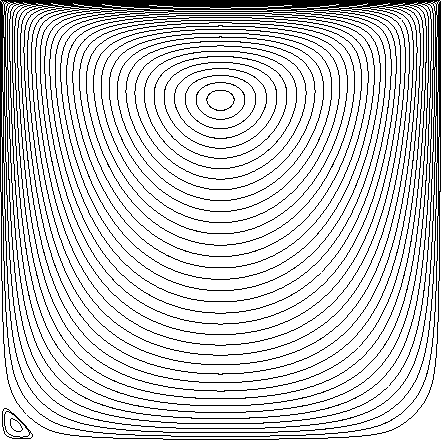
\includegraphics[width=0.5\textwidth]{figs/eddies1.png}
\end{center}
\end{itemize}
\end{frame}


\begin{frame}{fluid equations}

\begin{itemize}
\item FIXME
\end{itemize}
\end{frame}


\begin{frame}{the Stokes equations}

\hfill 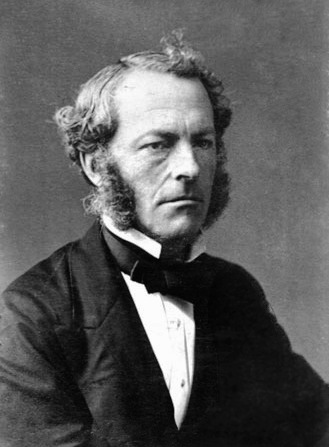
\includegraphics[width=0.25\textwidth]{figs/people/gstokes.jpg}

\vspace{-20mm}
\begin{itemize}
\item FIXME
\end{itemize}
\end{frame}


\begin{frame}{about the eddies}

\hfill 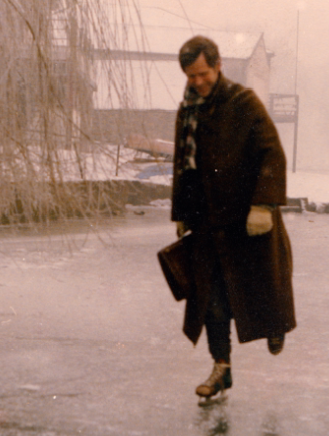
\includegraphics[width=0.25\textwidth]{figs/people/hkmoffatt.png}

%\vspace{-20mm}
\begin{itemize}
\item FIXME
\end{itemize}

\hfill 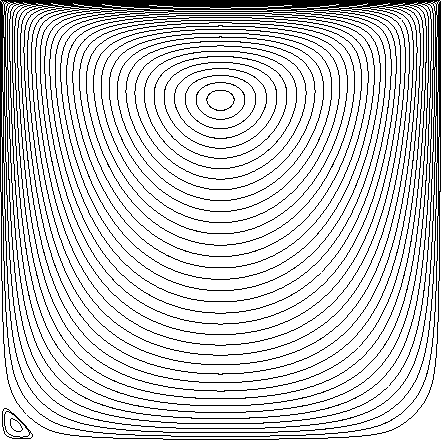
\includegraphics[width=0.25\textwidth]{figs/eddies1.png} 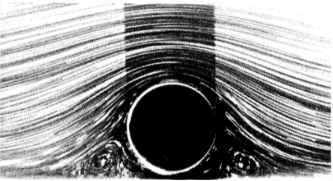
\includegraphics[width=0.25\textwidth]{figs/cylindereddies.pdf}
\end{frame}


\section{discretization, matrices, and solvers}

\begin{frame}{FIXME}

\begin{itemize}
\item FIXME
\end{itemize}
\end{frame}

\begin{frame}{mesh for Stokes}

\begin{itemize}
\item FIXME
\begin{center}
% created by command line:
%   petsc2tikz.py --nodesize 0.0 --dirichletsize 0.05 --scale 6.0 gradedcorners -o gradedcorners.tikz
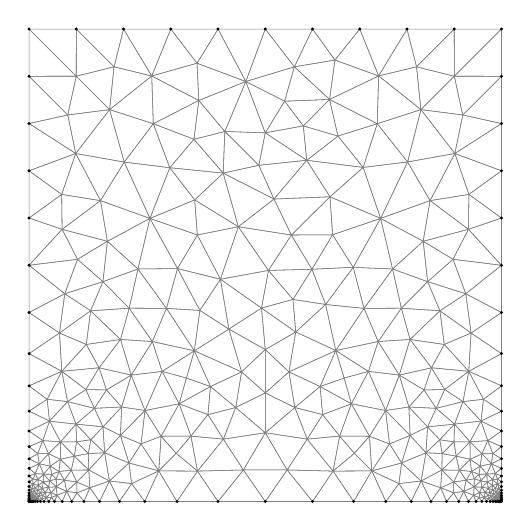
\begin{tikzpicture}[scale=6.000000]
  \draw[gray,very thin] (0.506761,0.489081) -- (0.443002,0.581530) -- (0.405103,0.470408) -- (0.506761,0.489081) ;
  \draw[gray,very thin] (1.000000,1.000000) -- (0.900000,1.000000) -- (0.900122,0.900122) -- (1.000000,1.000000) ;
  \draw[gray,very thin] (0.000000,1.000000) -- (0.000000,0.900000) -- (0.099878,0.900122) -- (0.000000,1.000000) ;
  \draw[gray,very thin] (0.000000,1.000000) -- (0.099878,0.900122) -- (0.100000,1.000000) -- (0.000000,1.000000) ;
  \draw[gray,very thin] (1.000000,1.000000) -- (0.900122,0.900122) -- (1.000000,0.900000) -- (1.000000,1.000000) ;
  \draw[gray,very thin] (0.997480,0.000000) -- (0.998892,0.000000) -- (0.998938,0.001062) -- (0.997480,0.000000) ;
  \draw[gray,very thin] (0.000000,0.002520) -- (0.000000,0.001108) -- (0.001062,0.001062) -- (0.000000,0.002520) ;
  \draw[gray,very thin] (0.001108,0.000000) -- (0.002520,0.000000) -- (0.001062,0.001062) -- (0.001108,0.000000) ;
  \draw[gray,very thin] (1.000000,0.001108) -- (1.000000,0.002520) -- (0.998938,0.001062) -- (1.000000,0.001108) ;
  \draw[gray,very thin] (0.126373,0.066725) -- (0.170147,0.043352) -- (0.159924,0.103139) -- (0.126373,0.066725) ;
  \draw[gray,very thin] (0.933275,0.126373) -- (0.956648,0.170147) -- (0.900655,0.163795) -- (0.933275,0.126373) ;
  \draw[gray,very thin] (0.873627,0.066725) -- (0.840076,0.103139) -- (0.829853,0.043352) -- (0.873627,0.066725) ;
  \draw[gray,very thin] (0.066725,0.126373) -- (0.099345,0.163795) -- (0.043352,0.170147) -- (0.066725,0.126373) ;
  \draw[gray,very thin] (0.356228,0.564091) -- (0.405103,0.470408) -- (0.443002,0.581530) -- (0.356228,0.564091) ;
  \draw[gray,very thin] (0.506761,0.489081) -- (0.405103,0.470408) -- (0.491910,0.409379) -- (0.506761,0.489081) ;
  \draw[gray,very thin] (0.769416,0.492148) -- (0.709073,0.408713) -- (0.788068,0.409160) -- (0.769416,0.492148) ;
  \draw[gray,very thin] (0.230584,0.492148) -- (0.211932,0.409160) -- (0.290927,0.408713) -- (0.230584,0.492148) ;
  \draw[gray,very thin] (0.707143,0.707143) -- (0.744101,0.599200) -- (0.801244,0.718639) -- (0.707143,0.707143) ;
  \draw[gray,very thin] (0.297812,0.706494) -- (0.201468,0.718418) -- (0.255899,0.599200) -- (0.297812,0.706494) ;
  \draw[gray,very thin] (0.422899,0.364854) -- (0.491910,0.409379) -- (0.405103,0.470408) -- (0.422899,0.364854) ;
  \draw[gray,very thin] (0.806560,0.139960) -- (0.754616,0.192571) -- (0.762958,0.121821) -- (0.806560,0.139960) ;
  \draw[gray,very thin] (0.193440,0.139960) -- (0.237042,0.121821) -- (0.245384,0.192571) -- (0.193440,0.139960) ;
  \draw[gray,very thin] (0.769416,0.492148) -- (0.686103,0.495641) -- (0.709073,0.408713) -- (0.769416,0.492148) ;
  \draw[gray,very thin] (0.230584,0.492148) -- (0.290927,0.408713) -- (0.314207,0.493062) -- (0.230584,0.492148) ;
  \draw[gray,very thin] (0.000000,0.191230) -- (0.000000,0.149200) -- (0.043352,0.170147) -- (0.000000,0.191230) ;
  \draw[gray,very thin] (0.808770,0.000000) -- (0.850800,0.000000) -- (0.829853,0.043352) -- (0.808770,0.000000) ;
  \draw[gray,very thin] (1.000000,0.149200) -- (1.000000,0.191230) -- (0.956648,0.170147) -- (1.000000,0.149200) ;
  \draw[gray,very thin] (0.149200,0.000000) -- (0.191230,0.000000) -- (0.170147,0.043352) -- (0.149200,0.000000) ;
  \draw[gray,very thin] (0.848779,0.636822) -- (0.801244,0.718639) -- (0.744101,0.599200) -- (0.848779,0.636822) ;
  \draw[gray,very thin] (0.151221,0.636822) -- (0.255899,0.599200) -- (0.201468,0.718418) -- (0.151221,0.636822) ;
  \draw[gray,very thin] (0.909668,0.000000) -- (0.929981,0.000000) -- (0.920152,0.021463) -- (0.909668,0.000000) ;
  \draw[gray,very thin] (0.000000,0.090332) -- (0.000000,0.070019) -- (0.021463,0.079848) -- (0.000000,0.090332) ;
  \draw[gray,very thin] (0.070019,0.000000) -- (0.090332,0.000000) -- (0.079856,0.021476) -- (0.070019,0.000000) ;
  \draw[gray,very thin] (1.000000,0.070019) -- (1.000000,0.090332) -- (0.978524,0.079856) -- (1.000000,0.070019) ;
  \draw[gray,very thin] (0.997480,0.000000) -- (0.998938,0.001062) -- (0.998052,0.001948) -- (0.997480,0.000000) ;
  \draw[gray,very thin] (0.000000,0.002520) -- (0.001062,0.001062) -- (0.001948,0.001948) -- (0.000000,0.002520) ;
  \draw[gray,very thin] (0.002520,0.000000) -- (0.001948,0.001948) -- (0.001062,0.001062) -- (0.002520,0.000000) ;
  \draw[gray,very thin] (1.000000,0.002520) -- (0.998052,0.001948) -- (0.998938,0.001062) -- (1.000000,0.002520) ;
  \draw[gray,very thin] (0.126373,0.066725) -- (0.089376,0.066358) -- (0.101110,0.041347) -- (0.126373,0.066725) ;
  \draw[gray,very thin] (0.933275,0.126373) -- (0.933642,0.089376) -- (0.958653,0.101110) -- (0.933275,0.126373) ;
  \draw[gray,very thin] (0.873627,0.066725) -- (0.898890,0.041347) -- (0.910613,0.066339) -- (0.873627,0.066725) ;
  \draw[gray,very thin] (0.066725,0.126373) -- (0.041347,0.101110) -- (0.066339,0.089387) -- (0.066725,0.126373) ;
  \draw[gray,very thin] (0.015695,0.016013) -- (0.008612,0.015907) -- (0.012276,0.011427) -- (0.015695,0.016013) ;
  \draw[gray,very thin] (0.983987,0.015695) -- (0.984093,0.008612) -- (0.988573,0.012276) -- (0.983987,0.015695) ;
  \draw[gray,very thin] (0.500000,1.000000) -- (0.400000,1.000000) -- (0.458784,0.888924) -- (0.500000,1.000000) ;
  \draw[gray,very thin] (0.400000,1.000000) -- (0.355555,0.927680) -- (0.458784,0.888924) -- (0.400000,1.000000) ;
  \draw[gray,very thin] (0.850800,0.000000) -- (0.871185,0.029065) -- (0.829853,0.043352) -- (0.850800,0.000000) ;
  \draw[gray,very thin] (0.000000,0.149200) -- (0.029065,0.128815) -- (0.043352,0.170147) -- (0.000000,0.149200) ;
  \draw[gray,very thin] (1.000000,0.149200) -- (0.956648,0.170147) -- (0.970935,0.128815) -- (1.000000,0.149200) ;
  \draw[gray,very thin] (0.149200,0.000000) -- (0.170147,0.043352) -- (0.128815,0.029065) -- (0.149200,0.000000) ;
  \draw[gray,very thin] (0.518409,0.640157) -- (0.555190,0.564038) -- (0.636961,0.644934) -- (0.518409,0.640157) ;
  \draw[gray,very thin] (0.991692,0.004654) -- (0.988238,0.007123) -- (0.988952,0.002842) -- (0.991692,0.004654) ;
  \draw[gray,very thin] (0.004654,0.008308) -- (0.007123,0.011762) -- (0.002842,0.011048) -- (0.004654,0.008308) ;
  \draw[gray,very thin] (0.995370,0.008332) -- (0.997162,0.011052) -- (0.993683,0.011852) -- (0.995370,0.008332) ;
  \draw[gray,very thin] (0.008332,0.004630) -- (0.011052,0.002838) -- (0.011852,0.006317) -- (0.008332,0.004630) ;
  \draw[gray,very thin] (0.518409,0.640157) -- (0.410877,0.695068) -- (0.443002,0.581530) -- (0.518409,0.640157) ;
  \draw[gray,very thin] (0.410877,0.695068) -- (0.350647,0.638383) -- (0.443002,0.581530) -- (0.410877,0.695068) ;
  \draw[gray,very thin] (0.000000,0.070019) -- (0.013279,0.059149) -- (0.021463,0.079848) -- (0.000000,0.070019) ;
  \draw[gray,very thin] (0.929981,0.000000) -- (0.940851,0.013279) -- (0.920152,0.021463) -- (0.929981,0.000000) ;
  \draw[gray,very thin] (1.000000,0.070019) -- (0.978524,0.079856) -- (0.986701,0.059162) -- (1.000000,0.070019) ;
  \draw[gray,very thin] (0.070019,0.000000) -- (0.079856,0.021476) -- (0.059162,0.013299) -- (0.070019,0.000000) ;
  \draw[gray,very thin] (0.000000,0.244787) -- (0.038250,0.216311) -- (0.069289,0.275584) -- (0.000000,0.244787) ;
  \draw[gray,very thin] (0.755213,0.000000) -- (0.782865,0.037854) -- (0.725447,0.064822) -- (0.755213,0.000000) ;
  \draw[gray,very thin] (0.244787,0.000000) -- (0.274553,0.064822) -- (0.217135,0.037854) -- (0.244787,0.000000) ;
  \draw[gray,very thin] (1.000000,0.244787) -- (0.930711,0.275584) -- (0.961750,0.216311) -- (1.000000,0.244787) ;
  \draw[gray,very thin] (0.933275,0.126373) -- (0.904080,0.095920) -- (0.933642,0.089376) -- (0.933275,0.126373) ;
  \draw[gray,very thin] (0.126373,0.066725) -- (0.095920,0.095920) -- (0.089376,0.066358) -- (0.126373,0.066725) ;
  \draw[gray,very thin] (0.873627,0.066725) -- (0.910613,0.066339) -- (0.904080,0.095920) -- (0.873627,0.066725) ;
  \draw[gray,very thin] (0.066725,0.126373) -- (0.066339,0.089387) -- (0.095920,0.095920) -- (0.066725,0.126373) ;
  \draw[gray,very thin] (0.506761,0.489081) -- (0.598761,0.491607) -- (0.555190,0.564038) -- (0.506761,0.489081) ;
  \draw[gray,very thin] (0.126373,0.066725) -- (0.101110,0.041347) -- (0.128815,0.029065) -- (0.126373,0.066725) ;
  \draw[gray,very thin] (0.933275,0.126373) -- (0.958653,0.101110) -- (0.970935,0.128815) -- (0.933275,0.126373) ;
  \draw[gray,very thin] (0.066725,0.126373) -- (0.029065,0.128815) -- (0.041347,0.101110) -- (0.066725,0.126373) ;
  \draw[gray,very thin] (0.873627,0.066725) -- (0.871185,0.029065) -- (0.898890,0.041347) -- (0.873627,0.066725) ;
  \draw[gray,very thin] (0.081512,0.211465) -- (0.069289,0.275584) -- (0.038250,0.216311) -- (0.081512,0.211465) ;
  \draw[gray,very thin] (0.788535,0.081512) -- (0.725447,0.064822) -- (0.782865,0.037854) -- (0.788535,0.081512) ;
  \draw[gray,very thin] (0.918488,0.211465) -- (0.961750,0.216311) -- (0.930711,0.275584) -- (0.918488,0.211465) ;
  \draw[gray,very thin] (0.211465,0.081512) -- (0.217135,0.037854) -- (0.274553,0.064822) -- (0.211465,0.081512) ;
  \draw[gray,very thin] (0.992126,0.008015) -- (0.988238,0.007123) -- (0.991692,0.004654) -- (0.992126,0.008015) ;
  \draw[gray,very thin] (0.008015,0.007874) -- (0.007123,0.011762) -- (0.004654,0.008308) -- (0.008015,0.007874) ;
  \draw[gray,very thin] (0.992126,0.008015) -- (0.995370,0.008332) -- (0.993683,0.011852) -- (0.992126,0.008015) ;
  \draw[gray,very thin] (0.008015,0.007874) -- (0.008332,0.004630) -- (0.011852,0.006317) -- (0.008015,0.007874) ;
  \draw[gray,very thin] (0.211465,0.081512) -- (0.159924,0.103139) -- (0.170147,0.043352) -- (0.211465,0.081512) ;
  \draw[gray,very thin] (0.918488,0.211465) -- (0.900655,0.163795) -- (0.956648,0.170147) -- (0.918488,0.211465) ;
  \draw[gray,very thin] (0.788535,0.081512) -- (0.829853,0.043352) -- (0.840076,0.103139) -- (0.788535,0.081512) ;
  \draw[gray,very thin] (0.081512,0.211465) -- (0.043352,0.170147) -- (0.099345,0.163795) -- (0.081512,0.211465) ;
  \draw[gray,very thin] (0.016188,0.007692) -- (0.020526,0.011427) -- (0.012276,0.011427) -- (0.016188,0.007692) ;
  \draw[gray,very thin] (0.992308,0.016188) -- (0.988573,0.020526) -- (0.988573,0.012276) -- (0.992308,0.016188) ;
  \draw[gray,very thin] (0.000000,0.800000) -- (0.000000,0.700000) -- (0.098767,0.736564) -- (0.000000,0.800000) ;
  \draw[gray,very thin] (1.000000,0.700000) -- (1.000000,0.800000) -- (0.901233,0.736564) -- (1.000000,0.700000) ;
  \draw[gray,very thin] (0.422899,0.364854) -- (0.349821,0.318968) -- (0.449897,0.274319) -- (0.422899,0.364854) ;
  \draw[gray,very thin] (0.564452,0.358804) -- (0.550103,0.274319) -- (0.649199,0.319495) -- (0.564452,0.358804) ;
  \draw[gray,very thin] (0.196011,0.200038) -- (0.193440,0.139960) -- (0.245384,0.192571) -- (0.196011,0.200038) ;
  \draw[gray,very thin] (0.803989,0.200038) -- (0.754616,0.192571) -- (0.806560,0.139960) -- (0.803989,0.200038) ;
  \draw[gray,very thin] (0.383988,0.243301) -- (0.449897,0.274319) -- (0.349821,0.318968) -- (0.383988,0.243301) ;
  \draw[gray,very thin] (0.616012,0.243301) -- (0.649199,0.319495) -- (0.550103,0.274319) -- (0.616012,0.243301) ;
  \draw[gray,very thin] (0.506761,0.489081) -- (0.558668,0.427732) -- (0.598761,0.491607) -- (0.506761,0.489081) ;
  \draw[gray,very thin] (0.148245,0.283041) -- (0.216307,0.267498) -- (0.193556,0.342973) -- (0.148245,0.283041) ;
  \draw[gray,very thin] (0.851755,0.283041) -- (0.806444,0.342973) -- (0.783693,0.267498) -- (0.851755,0.283041) ;
  \draw[gray,very thin] (0.116216,0.000000) -- (0.128815,0.029065) -- (0.101389,0.018304) -- (0.116216,0.000000) ;
  \draw[gray,very thin] (1.000000,0.116216) -- (0.970935,0.128815) -- (0.981696,0.101389) -- (1.000000,0.116216) ;
  \draw[gray,very thin] (0.000000,0.116216) -- (0.018304,0.101389) -- (0.029065,0.128815) -- (0.000000,0.116216) ;
  \draw[gray,very thin] (0.883784,0.000000) -- (0.898611,0.018304) -- (0.871185,0.029065) -- (0.883784,0.000000) ;
  \draw[gray,very thin] (0.718342,0.275393) -- (0.754616,0.192571) -- (0.783693,0.267498) -- (0.718342,0.275393) ;
  \draw[gray,very thin] (0.281658,0.275393) -- (0.216307,0.267498) -- (0.245384,0.192571) -- (0.281658,0.275393) ;
  \draw[gray,very thin] (0.851755,0.283041) -- (0.930711,0.275584) -- (0.878861,0.332361) -- (0.851755,0.283041) ;
  \draw[gray,very thin] (0.148245,0.283041) -- (0.121139,0.332361) -- (0.069289,0.275584) -- (0.148245,0.283041) ;
  \draw[gray,very thin] (0.850800,0.000000) -- (0.883784,0.000000) -- (0.871185,0.029065) -- (0.850800,0.000000) ;
  \draw[gray,very thin] (0.000000,0.149200) -- (0.000000,0.116216) -- (0.029065,0.128815) -- (0.000000,0.149200) ;
  \draw[gray,very thin] (1.000000,0.116216) -- (1.000000,0.149200) -- (0.970935,0.128815) -- (1.000000,0.116216) ;
  \draw[gray,very thin] (0.116216,0.000000) -- (0.149200,0.000000) -- (0.128815,0.029065) -- (0.116216,0.000000) ;
  \draw[gray,very thin] (0.803989,0.200038) -- (0.783693,0.267498) -- (0.754616,0.192571) -- (0.803989,0.200038) ;
  \draw[gray,very thin] (0.196011,0.200038) -- (0.245384,0.192571) -- (0.216307,0.267498) -- (0.196011,0.200038) ;
  \draw[gray,very thin] (0.686966,0.000000) -- (0.755213,0.000000) -- (0.725447,0.064822) -- (0.686966,0.000000) ;
  \draw[gray,very thin] (0.000000,0.313034) -- (0.000000,0.244787) -- (0.069289,0.275584) -- (0.000000,0.313034) ;
  \draw[gray,very thin] (1.000000,0.244787) -- (1.000000,0.313034) -- (0.930711,0.275584) -- (1.000000,0.244787) ;
  \draw[gray,very thin] (0.244787,0.000000) -- (0.313034,0.000000) -- (0.274553,0.064822) -- (0.244787,0.000000) ;
  \draw[gray,very thin] (0.873627,0.066725) -- (0.829853,0.043352) -- (0.871185,0.029065) -- (0.873627,0.066725) ;
  \draw[gray,very thin] (0.066725,0.126373) -- (0.043352,0.170147) -- (0.029065,0.128815) -- (0.066725,0.126373) ;
  \draw[gray,very thin] (0.933275,0.126373) -- (0.970935,0.128815) -- (0.956648,0.170147) -- (0.933275,0.126373) ;
  \draw[gray,very thin] (0.126373,0.066725) -- (0.128815,0.029065) -- (0.170147,0.043352) -- (0.126373,0.066725) ;
  \draw[gray,very thin] (0.518409,0.640157) -- (0.636961,0.644934) -- (0.587744,0.722210) -- (0.518409,0.640157) ;
  \draw[gray,very thin] (0.148245,0.283041) -- (0.193556,0.342973) -- (0.121139,0.332361) -- (0.148245,0.283041) ;
  \draw[gray,very thin] (0.851755,0.283041) -- (0.878861,0.332361) -- (0.806444,0.342973) -- (0.851755,0.283041) ;
  \draw[gray,very thin] (0.359290,0.848866) -- (0.458784,0.888924) -- (0.355555,0.927680) -- (0.359290,0.848866) ;
  \draw[gray,very thin] (0.800000,1.000000) -- (0.700000,1.000000) -- (0.739957,0.900758) -- (0.800000,1.000000) ;
  \draw[gray,very thin] (0.300000,1.000000) -- (0.200000,1.000000) -- (0.259701,0.900609) -- (0.300000,1.000000) ;
  \draw[gray,very thin] (0.081512,0.211465) -- (0.120213,0.236954) -- (0.069289,0.275584) -- (0.081512,0.211465) ;
  \draw[gray,very thin] (0.788535,0.081512) -- (0.762958,0.121821) -- (0.725447,0.064822) -- (0.788535,0.081512) ;
  \draw[gray,very thin] (0.211465,0.081512) -- (0.274553,0.064822) -- (0.237042,0.121821) -- (0.211465,0.081512) ;
  \draw[gray,very thin] (0.918488,0.211465) -- (0.930711,0.275584) -- (0.879787,0.236954) -- (0.918488,0.211465) ;
  \draw[gray,very thin] (0.627709,0.416999) -- (0.709073,0.408713) -- (0.686103,0.495641) -- (0.627709,0.416999) ;
  \draw[gray,very thin] (0.361627,0.404497) -- (0.314207,0.493062) -- (0.290927,0.408713) -- (0.361627,0.404497) ;
  \draw[gray,very thin] (0.000000,0.000000) -- (0.001108,0.000000) -- (0.001062,0.001062) -- (0.000000,0.000000) ;
  \draw[gray,very thin] (0.000000,0.000000) -- (0.001062,0.001062) -- (0.000000,0.001108) -- (0.000000,0.000000) ;
  \draw[gray,very thin] (1.000000,0.000000) -- (0.998938,0.001062) -- (0.998892,0.000000) -- (1.000000,0.000000) ;
  \draw[gray,very thin] (1.000000,0.000000) -- (1.000000,0.001108) -- (0.998938,0.001062) -- (1.000000,0.000000) ;
  \draw[gray,very thin] (0.843477,0.157971) -- (0.840076,0.103139) -- (0.869259,0.130741) -- (0.843477,0.157971) ;
  \draw[gray,very thin] (0.156523,0.157971) -- (0.099345,0.163795) -- (0.130741,0.130741) -- (0.156523,0.157971) ;
  \draw[gray,very thin] (0.843477,0.157971) -- (0.869259,0.130741) -- (0.900655,0.163795) -- (0.843477,0.157971) ;
  \draw[gray,very thin] (0.156523,0.157971) -- (0.130741,0.130741) -- (0.159924,0.103139) -- (0.156523,0.157971) ;
  \draw[gray,very thin] (0.054079,0.000000) -- (0.059162,0.013299) -- (0.047275,0.008174) -- (0.054079,0.000000) ;
  \draw[gray,very thin] (1.000000,0.054079) -- (0.986701,0.059162) -- (0.991826,0.047275) -- (1.000000,0.054079) ;
  \draw[gray,very thin] (0.945921,0.000000) -- (0.952728,0.008169) -- (0.940851,0.013279) -- (0.945921,0.000000) ;
  \draw[gray,very thin] (0.000000,0.054079) -- (0.008169,0.047272) -- (0.013279,0.059149) -- (0.000000,0.054079) ;
  \draw[gray,very thin] (0.972100,0.027900) -- (0.969845,0.041415) -- (0.958562,0.030128) -- (0.972100,0.027900) ;
  \draw[gray,very thin] (0.027900,0.027900) -- (0.041415,0.030155) -- (0.030128,0.041438) -- (0.027900,0.027900) ;
  \draw[gray,very thin] (0.995331,0.020278) -- (0.994283,0.027443) -- (0.988573,0.020526) -- (0.995331,0.020278) ;
  \draw[gray,very thin] (0.979769,0.004822) -- (0.978442,0.011295) -- (0.972629,0.005902) -- (0.979769,0.004822) ;
  \draw[gray,very thin] (0.004822,0.020231) -- (0.011295,0.021558) -- (0.005902,0.027371) -- (0.004822,0.020231) ;
  \draw[gray,very thin] (0.020278,0.004669) -- (0.027443,0.005717) -- (0.020526,0.011427) -- (0.020278,0.004669) ;
  \draw[gray,very thin] (0.000000,0.070019) -- (0.000000,0.054079) -- (0.013279,0.059149) -- (0.000000,0.070019) ;
  \draw[gray,very thin] (0.929981,0.000000) -- (0.945921,0.000000) -- (0.940851,0.013279) -- (0.929981,0.000000) ;
  \draw[gray,very thin] (0.054079,0.000000) -- (0.070019,0.000000) -- (0.059162,0.013299) -- (0.054079,0.000000) ;
  \draw[gray,very thin] (1.000000,0.054079) -- (1.000000,0.070019) -- (0.986701,0.059162) -- (1.000000,0.054079) ;
  \draw[gray,very thin] (0.518409,0.640157) -- (0.486386,0.711656) -- (0.410877,0.695068) -- (0.518409,0.640157) ;
  \draw[gray,very thin] (0.642512,0.564557) -- (0.636961,0.644934) -- (0.555190,0.564038) -- (0.642512,0.564557) ;
  \draw[gray,very thin] (0.356228,0.564091) -- (0.443002,0.581530) -- (0.350647,0.638383) -- (0.356228,0.564091) ;
  \draw[gray,very thin] (0.968895,0.057971) -- (0.978524,0.079856) -- (0.954900,0.074892) -- (0.968895,0.057971) ;
  \draw[gray,very thin] (0.057971,0.031105) -- (0.079856,0.021476) -- (0.074892,0.045100) -- (0.057971,0.031105) ;
  \draw[gray,very thin] (0.031017,0.057912) -- (0.044972,0.074820) -- (0.021463,0.079848) -- (0.031017,0.057912) ;
  \draw[gray,very thin] (0.942088,0.031017) -- (0.925180,0.044972) -- (0.920152,0.021463) -- (0.942088,0.031017) ;
  \draw[gray,very thin] (0.598761,0.491607) -- (0.627709,0.416999) -- (0.686103,0.495641) -- (0.598761,0.491607) ;
  \draw[gray,very thin] (0.405103,0.470408) -- (0.314207,0.493062) -- (0.361627,0.404497) -- (0.405103,0.470408) ;
  \draw[gray,very thin] (0.101110,0.041347) -- (0.101389,0.018304) -- (0.128815,0.029065) -- (0.101110,0.041347) ;
  \draw[gray,very thin] (0.958653,0.101110) -- (0.981696,0.101389) -- (0.970935,0.128815) -- (0.958653,0.101110) ;
  \draw[gray,very thin] (0.041347,0.101110) -- (0.029065,0.128815) -- (0.018304,0.101389) -- (0.041347,0.101110) ;
  \draw[gray,very thin] (0.898890,0.041347) -- (0.871185,0.029065) -- (0.898611,0.018304) -- (0.898890,0.041347) ;
  \draw[gray,very thin] (0.031017,0.057912) -- (0.021463,0.079848) -- (0.013279,0.059149) -- (0.031017,0.057912) ;
  \draw[gray,very thin] (0.942088,0.031017) -- (0.920152,0.021463) -- (0.940851,0.013279) -- (0.942088,0.031017) ;
  \draw[gray,very thin] (0.968895,0.057971) -- (0.986701,0.059162) -- (0.978524,0.079856) -- (0.968895,0.057971) ;
  \draw[gray,very thin] (0.057971,0.031105) -- (0.059162,0.013299) -- (0.079856,0.021476) -- (0.057971,0.031105) ;
  \draw[gray,very thin] (0.986742,0.000000) -- (0.990465,0.000000) -- (0.988952,0.002842) -- (0.986742,0.000000) ;
  \draw[gray,very thin] (0.000000,0.013258) -- (0.000000,0.009535) -- (0.002842,0.011048) -- (0.000000,0.013258) ;
  \draw[gray,very thin] (0.009535,0.000000) -- (0.013258,0.000000) -- (0.011052,0.002838) -- (0.009535,0.000000) ;
  \draw[gray,very thin] (1.000000,0.009535) -- (1.000000,0.013258) -- (0.997162,0.011052) -- (1.000000,0.009535) ;
  \draw[gray,very thin] (0.500000,0.780314) -- (0.458784,0.888924) -- (0.414367,0.783231) -- (0.500000,0.780314) ;
  \draw[gray,very thin] (0.359290,0.848866) -- (0.414367,0.783231) -- (0.458784,0.888924) -- (0.359290,0.848866) ;
  \draw[gray,very thin] (0.642512,0.564557) -- (0.555190,0.564038) -- (0.598761,0.491607) -- (0.642512,0.564557) ;
  \draw[gray,very thin] (0.500000,1.000000) -- (0.458784,0.888924) -- (0.561589,0.920061) -- (0.500000,1.000000) ;
  \draw[gray,very thin] (1.000000,0.004320) -- (1.000000,0.006613) -- (0.997870,0.005466) -- (1.000000,0.004320) ;
  \draw[gray,very thin] (0.000000,0.006613) -- (0.000000,0.004320) -- (0.002130,0.005466) -- (0.000000,0.006613) ;
  \draw[gray,very thin] (0.993387,0.000000) -- (0.995680,0.000000) -- (0.994534,0.002130) -- (0.993387,0.000000) ;
  \draw[gray,very thin] (0.004320,0.000000) -- (0.006613,0.000000) -- (0.005466,0.002130) -- (0.004320,0.000000) ;
  \draw[gray,very thin] (0.769416,0.492148) -- (0.744101,0.599200) -- (0.686103,0.495641) -- (0.769416,0.492148) ;
  \draw[gray,very thin] (0.230584,0.492148) -- (0.314207,0.493062) -- (0.255899,0.599200) -- (0.230584,0.492148) ;
  \draw[gray,very thin] (0.829497,0.829497) -- (0.801244,0.718639) -- (0.901233,0.736564) -- (0.829497,0.829497) ;
  \draw[gray,very thin] (0.170503,0.829497) -- (0.098767,0.736564) -- (0.201468,0.718418) -- (0.170503,0.829497) ;
  \draw[gray,very thin] (0.930711,0.275584) -- (0.935657,0.356517) -- (0.878861,0.332361) -- (0.930711,0.275584) ;
  \draw[gray,very thin] (0.069289,0.275584) -- (0.121139,0.332361) -- (0.064343,0.356517) -- (0.069289,0.275584) ;
  \draw[gray,very thin] (0.015695,0.016013) -- (0.011295,0.021558) -- (0.008612,0.015907) -- (0.015695,0.016013) ;
  \draw[gray,very thin] (0.983987,0.015695) -- (0.978442,0.011295) -- (0.984093,0.008612) -- (0.983987,0.015695) ;
  \draw[gray,very thin] (0.564452,0.358804) -- (0.491910,0.409379) -- (0.500000,0.321556) -- (0.564452,0.358804) ;
  \draw[gray,very thin] (0.686966,0.000000) -- (0.725447,0.064822) -- (0.643483,0.064343) -- (0.686966,0.000000) ;
  \draw[gray,very thin] (0.313034,0.000000) -- (0.356517,0.064343) -- (0.274553,0.064822) -- (0.313034,0.000000) ;
  \draw[gray,very thin] (0.588723,0.131995) -- (0.546285,0.066737) -- (0.643483,0.064343) -- (0.588723,0.131995) ;
  \draw[gray,very thin] (0.411277,0.131995) -- (0.356517,0.064343) -- (0.453715,0.066737) -- (0.411277,0.131995) ;
  \draw[gray,very thin] (0.997480,0.000000) -- (0.998052,0.001948) -- (0.996490,0.001474) -- (0.997480,0.000000) ;
  \draw[gray,very thin] (0.000000,0.002520) -- (0.001948,0.001948) -- (0.001474,0.003510) -- (0.000000,0.002520) ;
  \draw[gray,very thin] (0.002520,0.000000) -- (0.003510,0.001474) -- (0.001948,0.001948) -- (0.002520,0.000000) ;
  \draw[gray,very thin] (1.000000,0.002520) -- (0.998526,0.003510) -- (0.998052,0.001948) -- (1.000000,0.002520) ;
  \draw[gray,very thin] (0.422899,0.364854) -- (0.405103,0.470408) -- (0.361627,0.404497) -- (0.422899,0.364854) ;
  \draw[gray,very thin] (0.707143,0.707143) -- (0.636961,0.644934) -- (0.744101,0.599200) -- (0.707143,0.707143) ;
  \draw[gray,very thin] (0.000000,0.313034) -- (0.069289,0.275584) -- (0.064343,0.356517) -- (0.000000,0.313034) ;
  \draw[gray,very thin] (1.000000,0.313034) -- (0.935657,0.356517) -- (0.930711,0.275584) -- (1.000000,0.313034) ;
  \draw[gray,very thin] (0.063517,0.063550) -- (0.089376,0.066358) -- (0.066339,0.089387) -- (0.063517,0.063550) ;
  \draw[gray,very thin] (0.936450,0.063517) -- (0.933642,0.089376) -- (0.910613,0.066339) -- (0.936450,0.063517) ;
  \draw[gray,very thin] (0.000000,0.800000) -- (0.098767,0.736564) -- (0.081988,0.818090) -- (0.000000,0.800000) ;
  \draw[gray,very thin] (1.000000,0.800000) -- (0.918012,0.818090) -- (0.901233,0.736564) -- (1.000000,0.800000) ;
  \draw[gray,very thin] (0.642512,0.564557) -- (0.686103,0.495641) -- (0.744101,0.599200) -- (0.642512,0.564557) ;
  \draw[gray,very thin] (0.356228,0.564091) -- (0.255899,0.599200) -- (0.314207,0.493062) -- (0.356228,0.564091) ;
  \draw[gray,very thin] (0.057971,0.031105) -- (0.046636,0.018745) -- (0.059162,0.013299) -- (0.057971,0.031105) ;
  \draw[gray,very thin] (0.968895,0.057971) -- (0.981255,0.046636) -- (0.986701,0.059162) -- (0.968895,0.057971) ;
  \draw[gray,very thin] (0.942088,0.031017) -- (0.940851,0.013279) -- (0.953373,0.018730) -- (0.942088,0.031017) ;
  \draw[gray,very thin] (0.031017,0.057912) -- (0.013279,0.059149) -- (0.018730,0.046627) -- (0.031017,0.057912) ;
  \draw[gray,very thin] (0.297812,0.706494) -- (0.410877,0.695068) -- (0.349065,0.766655) -- (0.297812,0.706494) ;
  \draw[gray,very thin] (0.642512,0.564557) -- (0.744101,0.599200) -- (0.636961,0.644934) -- (0.642512,0.564557) ;
  \draw[gray,very thin] (0.636022,0.850901) -- (0.737024,0.799617) -- (0.739957,0.900758) -- (0.636022,0.850901) ;
  \draw[gray,very thin] (0.359290,0.848866) -- (0.259701,0.900609) -- (0.262976,0.799617) -- (0.359290,0.848866) ;
  \draw[gray,very thin] (0.990465,0.000000) -- (0.991806,0.001925) -- (0.988952,0.002842) -- (0.990465,0.000000) ;
  \draw[gray,very thin] (0.000000,0.009535) -- (0.001925,0.008194) -- (0.002842,0.011048) -- (0.000000,0.009535) ;
  \draw[gray,very thin] (0.009535,0.000000) -- (0.011052,0.002838) -- (0.008199,0.001920) -- (0.009535,0.000000) ;
  \draw[gray,very thin] (1.000000,0.009535) -- (0.997162,0.011052) -- (0.998080,0.008199) -- (1.000000,0.009535) ;
  \draw[gray,very thin] (0.170503,0.829497) -- (0.201468,0.718418) -- (0.262976,0.799617) -- (0.170503,0.829497) ;
  \draw[gray,very thin] (0.829497,0.829497) -- (0.737024,0.799617) -- (0.801244,0.718639) -- (0.829497,0.829497) ;
  \draw[gray,very thin] (0.588723,0.131995) -- (0.562585,0.198911) -- (0.500000,0.145513) -- (0.588723,0.131995) ;
  \draw[gray,very thin] (0.411277,0.131995) -- (0.500000,0.145513) -- (0.437415,0.198911) -- (0.411277,0.131995) ;
  \draw[gray,very thin] (0.279459,0.138127) -- (0.237042,0.121821) -- (0.274553,0.064822) -- (0.279459,0.138127) ;
  \draw[gray,very thin] (0.851755,0.283041) -- (0.879787,0.236954) -- (0.930711,0.275584) -- (0.851755,0.283041) ;
  \draw[gray,very thin] (0.720541,0.138127) -- (0.725447,0.064822) -- (0.762958,0.121821) -- (0.720541,0.138127) ;
  \draw[gray,very thin] (0.148245,0.283041) -- (0.069289,0.275584) -- (0.120213,0.236954) -- (0.148245,0.283041) ;
  \draw[gray,very thin] (0.008612,0.015907) -- (0.007123,0.011762) -- (0.012276,0.011427) -- (0.008612,0.015907) ;
  \draw[gray,very thin] (0.984093,0.008612) -- (0.988238,0.007123) -- (0.988573,0.012276) -- (0.984093,0.008612) ;
  \draw[gray,very thin] (0.046636,0.018745) -- (0.047275,0.008174) -- (0.059162,0.013299) -- (0.046636,0.018745) ;
  \draw[gray,very thin] (0.981255,0.046636) -- (0.991826,0.047275) -- (0.986701,0.059162) -- (0.981255,0.046636) ;
  \draw[gray,very thin] (0.953373,0.018730) -- (0.940851,0.013279) -- (0.952728,0.008169) -- (0.953373,0.018730) ;
  \draw[gray,very thin] (0.018730,0.046627) -- (0.013279,0.059149) -- (0.008169,0.047272) -- (0.018730,0.046627) ;
  \draw[gray,very thin] (0.400000,0.000000) -- (0.356517,0.064343) -- (0.313034,0.000000) -- (0.400000,0.000000) ;
  \draw[gray,very thin] (0.600000,0.000000) -- (0.686966,0.000000) -- (0.643483,0.064343) -- (0.600000,0.000000) ;
  \draw[gray,very thin] (0.297812,0.706494) -- (0.350647,0.638383) -- (0.410877,0.695068) -- (0.297812,0.706494) ;
  \draw[gray,very thin] (0.003293,0.003293) -- (0.005466,0.002130) -- (0.005230,0.005230) -- (0.003293,0.003293) ;
  \draw[gray,very thin] (0.003293,0.003293) -- (0.005230,0.005230) -- (0.002130,0.005466) -- (0.003293,0.003293) ;
  \draw[gray,very thin] (0.996707,0.003293) -- (0.997870,0.005466) -- (0.994770,0.005230) -- (0.996707,0.003293) ;
  \draw[gray,very thin] (0.996707,0.003293) -- (0.994770,0.005230) -- (0.994534,0.002130) -- (0.996707,0.003293) ;
  \draw[gray,very thin] (0.290927,0.408713) -- (0.211932,0.409160) -- (0.260945,0.338574) -- (0.290927,0.408713) ;
  \draw[gray,very thin] (0.709073,0.408713) -- (0.738938,0.338637) -- (0.788068,0.409160) -- (0.709073,0.408713) ;
  \draw[gray,very thin] (0.130265,0.403688) -- (0.121139,0.332361) -- (0.193556,0.342973) -- (0.130265,0.403688) ;
  \draw[gray,very thin] (0.869735,0.403688) -- (0.806444,0.342973) -- (0.878861,0.332361) -- (0.869735,0.403688) ;
  \draw[gray,very thin] (0.992126,0.008015) -- (0.994770,0.005230) -- (0.995370,0.008332) -- (0.992126,0.008015) ;
  \draw[gray,very thin] (0.992126,0.008015) -- (0.991692,0.004654) -- (0.994770,0.005230) -- (0.992126,0.008015) ;
  \draw[gray,very thin] (0.008015,0.007874) -- (0.005230,0.005230) -- (0.008332,0.004630) -- (0.008015,0.007874) ;
  \draw[gray,very thin] (0.008015,0.007874) -- (0.004654,0.008308) -- (0.005230,0.005230) -- (0.008015,0.007874) ;
  \draw[gray,very thin] (0.000000,0.041569) -- (0.000000,0.031752) -- (0.008244,0.036661) -- (0.000000,0.041569) ;
  \draw[gray,very thin] (0.958431,0.000000) -- (0.968248,0.000000) -- (0.963339,0.008244) -- (0.958431,0.000000) ;
  \draw[gray,very thin] (0.031752,0.000000) -- (0.041569,0.000000) -- (0.036661,0.008244) -- (0.031752,0.000000) ;
  \draw[gray,very thin] (1.000000,0.031752) -- (1.000000,0.041569) -- (0.991756,0.036661) -- (1.000000,0.031752) ;
  \draw[gray,very thin] (0.500000,0.229843) -- (0.500000,0.145513) -- (0.562585,0.198911) -- (0.500000,0.229843) ;
  \draw[gray,very thin] (0.500000,0.229843) -- (0.437415,0.198911) -- (0.500000,0.145513) -- (0.500000,0.229843) ;
  \draw[gray,very thin] (1.000000,0.400000) -- (0.935657,0.356517) -- (1.000000,0.313034) -- (1.000000,0.400000) ;
  \draw[gray,very thin] (0.000000,0.400000) -- (0.000000,0.313034) -- (0.064343,0.356517) -- (0.000000,0.400000) ;
  \draw[gray,very thin] (1.000000,0.004320) -- (0.997870,0.005466) -- (0.998526,0.003510) -- (1.000000,0.004320) ;
  \draw[gray,very thin] (0.000000,0.004320) -- (0.001474,0.003510) -- (0.002130,0.005466) -- (0.000000,0.004320) ;
  \draw[gray,very thin] (0.004320,0.000000) -- (0.005466,0.002130) -- (0.003510,0.001474) -- (0.004320,0.000000) ;
  \draw[gray,very thin] (0.995680,0.000000) -- (0.996490,0.001474) -- (0.994534,0.002130) -- (0.995680,0.000000) ;
  \draw[gray,very thin] (0.015695,0.016013) -- (0.012276,0.011427) -- (0.020526,0.011427) -- (0.015695,0.016013) ;
  \draw[gray,very thin] (0.983987,0.015695) -- (0.988573,0.012276) -- (0.988573,0.020526) -- (0.983987,0.015695) ;
  \draw[gray,very thin] (0.400000,0.000000) -- (0.453715,0.066737) -- (0.356517,0.064343) -- (0.400000,0.000000) ;
  \draw[gray,very thin] (0.600000,0.000000) -- (0.643483,0.064343) -- (0.546285,0.066737) -- (0.600000,0.000000) ;
  \draw[gray,very thin] (0.057971,0.031105) -- (0.041415,0.030155) -- (0.046636,0.018745) -- (0.057971,0.031105) ;
  \draw[gray,very thin] (0.968895,0.057971) -- (0.969845,0.041415) -- (0.981255,0.046636) -- (0.968895,0.057971) ;
  \draw[gray,very thin] (0.031017,0.057912) -- (0.018730,0.046627) -- (0.030128,0.041438) -- (0.031017,0.057912) ;
  \draw[gray,very thin] (0.942088,0.031017) -- (0.953373,0.018730) -- (0.958562,0.030128) -- (0.942088,0.031017) ;
  \draw[gray,very thin] (0.193556,0.342973) -- (0.260945,0.338574) -- (0.211932,0.409160) -- (0.193556,0.342973) ;
  \draw[gray,very thin] (0.806444,0.342973) -- (0.788068,0.409160) -- (0.738938,0.338637) -- (0.806444,0.342973) ;
  \draw[gray,very thin] (0.996707,0.003293) -- (0.998052,0.001948) -- (0.998526,0.003510) -- (0.996707,0.003293) ;
  \draw[gray,very thin] (0.996707,0.003293) -- (0.996490,0.001474) -- (0.998052,0.001948) -- (0.996707,0.003293) ;
  \draw[gray,very thin] (0.003293,0.003293) -- (0.001948,0.001948) -- (0.003510,0.001474) -- (0.003293,0.003293) ;
  \draw[gray,very thin] (0.003293,0.003293) -- (0.001474,0.003510) -- (0.001948,0.001948) -- (0.003293,0.003293) ;
  \draw[gray,very thin] (0.081512,0.211465) -- (0.099345,0.163795) -- (0.138375,0.197184) -- (0.081512,0.211465) ;
  \draw[gray,very thin] (0.788535,0.081512) -- (0.840076,0.103139) -- (0.806560,0.139960) -- (0.788535,0.081512) ;
  \draw[gray,very thin] (0.918488,0.211465) -- (0.861625,0.197184) -- (0.900655,0.163795) -- (0.918488,0.211465) ;
  \draw[gray,very thin] (0.211465,0.081512) -- (0.193440,0.139960) -- (0.159924,0.103139) -- (0.211465,0.081512) ;
  \draw[gray,very thin] (0.987418,0.028691) -- (0.991756,0.036661) -- (0.980816,0.034285) -- (0.987418,0.028691) ;
  \draw[gray,very thin] (0.971351,0.013004) -- (0.965469,0.019654) -- (0.963339,0.008244) -- (0.971351,0.013004) ;
  \draw[gray,very thin] (0.028691,0.012582) -- (0.036661,0.008244) -- (0.034285,0.019184) -- (0.028691,0.012582) ;
  \draw[gray,very thin] (0.013004,0.028649) -- (0.019654,0.034531) -- (0.008244,0.036661) -- (0.013004,0.028649) ;
  \draw[gray,very thin] (0.600000,1.000000) -- (0.500000,1.000000) -- (0.561589,0.920061) -- (0.600000,1.000000) ;
  \draw[gray,very thin] (0.975952,0.000000) -- (0.981998,0.000000) -- (0.979769,0.004822) -- (0.975952,0.000000) ;
  \draw[gray,very thin] (0.000000,0.024048) -- (0.000000,0.018002) -- (0.004822,0.020231) -- (0.000000,0.024048) ;
  \draw[gray,very thin] (1.000000,0.018002) -- (1.000000,0.024048) -- (0.995331,0.020278) -- (1.000000,0.018002) ;
  \draw[gray,very thin] (0.018002,0.000000) -- (0.024048,0.000000) -- (0.020278,0.004669) -- (0.018002,0.000000) ;
  \draw[gray,very thin] (0.500000,0.780314) -- (0.540903,0.847349) -- (0.458784,0.888924) -- (0.500000,0.780314) ;
  \draw[gray,very thin] (0.297812,0.706494) -- (0.255899,0.599200) -- (0.350647,0.638383) -- (0.297812,0.706494) ;
  \draw[gray,very thin] (0.981998,0.000000) -- (0.984831,0.003635) -- (0.979769,0.004822) -- (0.981998,0.000000) ;
  \draw[gray,very thin] (0.018002,0.000000) -- (0.020278,0.004669) -- (0.015248,0.003439) -- (0.018002,0.000000) ;
  \draw[gray,very thin] (0.000000,0.018002) -- (0.003635,0.015169) -- (0.004822,0.020231) -- (0.000000,0.018002) ;
  \draw[gray,very thin] (1.000000,0.018002) -- (0.995331,0.020278) -- (0.996561,0.015248) -- (1.000000,0.018002) ;
  \draw[gray,very thin] (0.933275,0.126373) -- (0.899367,0.126083) -- (0.904080,0.095920) -- (0.933275,0.126373) ;
  \draw[gray,very thin] (0.126373,0.066725) -- (0.125404,0.101378) -- (0.095920,0.095920) -- (0.126373,0.066725) ;
  \draw[gray,very thin] (0.873627,0.066725) -- (0.904080,0.095920) -- (0.874511,0.101306) -- (0.873627,0.066725) ;
  \draw[gray,very thin] (0.066725,0.126373) -- (0.095920,0.095920) -- (0.100546,0.126183) -- (0.066725,0.126373) ;
  \draw[gray,very thin] (0.720541,0.138127) -- (0.762958,0.121821) -- (0.754616,0.192571) -- (0.720541,0.138127) ;
  \draw[gray,very thin] (0.279459,0.138127) -- (0.245384,0.192571) -- (0.237042,0.121821) -- (0.279459,0.138127) ;
  \draw[gray,very thin] (0.211465,0.081512) -- (0.170147,0.043352) -- (0.217135,0.037854) -- (0.211465,0.081512) ;
  \draw[gray,very thin] (0.918488,0.211465) -- (0.956648,0.170147) -- (0.961750,0.216311) -- (0.918488,0.211465) ;
  \draw[gray,very thin] (0.788535,0.081512) -- (0.782865,0.037854) -- (0.829853,0.043352) -- (0.788535,0.081512) ;
  \draw[gray,very thin] (0.081512,0.211465) -- (0.038250,0.216311) -- (0.043352,0.170147) -- (0.081512,0.211465) ;
  \draw[gray,very thin] (0.800000,1.000000) -- (0.739957,0.900758) -- (0.820102,0.920029) -- (0.800000,1.000000) ;
  \draw[gray,very thin] (0.200000,1.000000) -- (0.179898,0.920029) -- (0.259701,0.900609) -- (0.200000,1.000000) ;
  \draw[gray,very thin] (0.281658,0.275393) -- (0.260945,0.338574) -- (0.216307,0.267498) -- (0.281658,0.275393) ;
  \draw[gray,very thin] (0.718342,0.275393) -- (0.783693,0.267498) -- (0.738938,0.338637) -- (0.718342,0.275393) ;
  \draw[gray,very thin] (0.031752,0.000000) -- (0.036661,0.008244) -- (0.027443,0.005717) -- (0.031752,0.000000) ;
  \draw[gray,very thin] (1.000000,0.031752) -- (0.991756,0.036661) -- (0.994283,0.027443) -- (1.000000,0.031752) ;
  \draw[gray,very thin] (0.968248,0.000000) -- (0.972629,0.005902) -- (0.963339,0.008244) -- (0.968248,0.000000) ;
  \draw[gray,very thin] (0.000000,0.031752) -- (0.005902,0.027371) -- (0.008244,0.036661) -- (0.000000,0.031752) ;
  \draw[gray,very thin] (0.718342,0.275393) -- (0.682253,0.206807) -- (0.754616,0.192571) -- (0.718342,0.275393) ;
  \draw[gray,very thin] (0.281658,0.275393) -- (0.245384,0.192571) -- (0.317747,0.206807) -- (0.281658,0.275393) ;
  \draw[gray,very thin] (0.588723,0.131995) -- (0.500000,0.145513) -- (0.546285,0.066737) -- (0.588723,0.131995) ;
  \draw[gray,very thin] (0.411277,0.131995) -- (0.453715,0.066737) -- (0.500000,0.145513) -- (0.411277,0.131995) ;
  \draw[gray,very thin] (0.000000,0.900000) -- (0.000000,0.800000) -- (0.081988,0.818090) -- (0.000000,0.900000) ;
  \draw[gray,very thin] (1.000000,0.800000) -- (1.000000,0.900000) -- (0.918012,0.818090) -- (1.000000,0.800000) ;
  \draw[gray,very thin] (0.000000,0.900000) -- (0.081988,0.818090) -- (0.099878,0.900122) -- (0.000000,0.900000) ;
  \draw[gray,very thin] (1.000000,0.900000) -- (0.900122,0.900122) -- (0.918012,0.818090) -- (1.000000,0.900000) ;
  \draw[gray,very thin] (0.971351,0.013004) -- (0.976043,0.019163) -- (0.965469,0.019654) -- (0.971351,0.013004) ;
  \draw[gray,very thin] (0.013004,0.028649) -- (0.019163,0.023957) -- (0.019654,0.034531) -- (0.013004,0.028649) ;
  \draw[gray,very thin] (0.057971,0.031105) -- (0.043597,0.043624) -- (0.041415,0.030155) -- (0.057971,0.031105) ;
  \draw[gray,very thin] (0.968895,0.057971) -- (0.956376,0.043597) -- (0.969845,0.041415) -- (0.968895,0.057971) ;
  \draw[gray,very thin] (0.031017,0.057912) -- (0.030128,0.041438) -- (0.043597,0.043624) -- (0.031017,0.057912) ;
  \draw[gray,very thin] (0.942088,0.031017) -- (0.958562,0.030128) -- (0.956376,0.043597) -- (0.942088,0.031017) ;
  \draw[gray,very thin] (0.829497,0.829497) -- (0.739957,0.900758) -- (0.737024,0.799617) -- (0.829497,0.829497) ;
  \draw[gray,very thin] (0.170503,0.829497) -- (0.262976,0.799617) -- (0.259701,0.900609) -- (0.170503,0.829497) ;
  \draw[gray,very thin] (0.518409,0.640157) -- (0.587744,0.722210) -- (0.486386,0.711656) -- (0.518409,0.640157) ;
  \draw[gray,very thin] (0.500000,0.780314) -- (0.486386,0.711656) -- (0.587744,0.722210) -- (0.500000,0.780314) ;
  \draw[gray,very thin] (0.848779,0.636822) -- (0.901233,0.736564) -- (0.801244,0.718639) -- (0.848779,0.636822) ;
  \draw[gray,very thin] (0.151221,0.636822) -- (0.201468,0.718418) -- (0.098767,0.736564) -- (0.151221,0.636822) ;
  \draw[gray,very thin] (0.806560,0.139960) -- (0.840076,0.103139) -- (0.843477,0.157971) -- (0.806560,0.139960) ;
  \draw[gray,very thin] (0.138375,0.197184) -- (0.099345,0.163795) -- (0.156523,0.157971) -- (0.138375,0.197184) ;
  \draw[gray,very thin] (0.861625,0.197184) -- (0.843477,0.157971) -- (0.900655,0.163795) -- (0.861625,0.197184) ;
  \draw[gray,very thin] (0.193440,0.139960) -- (0.156523,0.157971) -- (0.159924,0.103139) -- (0.193440,0.139960) ;
  \draw[gray,very thin] (0.193556,0.342973) -- (0.216307,0.267498) -- (0.260945,0.338574) -- (0.193556,0.342973) ;
  \draw[gray,very thin] (0.806444,0.342973) -- (0.738938,0.338637) -- (0.783693,0.267498) -- (0.806444,0.342973) ;
  \draw[gray,very thin] (1.000000,0.500000) -- (0.930035,0.576058) -- (0.897437,0.512686) -- (1.000000,0.500000) ;
  \draw[gray,very thin] (0.000000,0.500000) -- (0.102563,0.512686) -- (0.069965,0.576058) -- (0.000000,0.500000) ;
  \draw[gray,very thin] (0.991692,0.004654) -- (0.988952,0.002842) -- (0.991806,0.001925) -- (0.991692,0.004654) ;
  \draw[gray,very thin] (0.004654,0.008308) -- (0.002842,0.011048) -- (0.001925,0.008194) -- (0.004654,0.008308) ;
  \draw[gray,very thin] (0.995370,0.008332) -- (0.998080,0.008199) -- (0.997162,0.011052) -- (0.995370,0.008332) ;
  \draw[gray,very thin] (0.008332,0.004630) -- (0.008199,0.001920) -- (0.011052,0.002838) -- (0.008332,0.004630) ;
  \draw[gray,very thin] (0.130265,0.403688) -- (0.193556,0.342973) -- (0.211932,0.409160) -- (0.130265,0.403688) ;
  \draw[gray,very thin] (0.869735,0.403688) -- (0.788068,0.409160) -- (0.806444,0.342973) -- (0.869735,0.403688) ;
  \draw[gray,very thin] (1.000000,0.500000) -- (0.897437,0.512686) -- (0.924410,0.439686) -- (1.000000,0.500000) ;
  \draw[gray,very thin] (0.000000,0.500000) -- (0.075590,0.439686) -- (0.102563,0.512686) -- (0.000000,0.500000) ;
  \draw[gray,very thin] (0.580470,0.794999) -- (0.636022,0.850901) -- (0.540903,0.847349) -- (0.580470,0.794999) ;
  \draw[gray,very thin] (0.564452,0.358804) -- (0.500000,0.321556) -- (0.550103,0.274319) -- (0.564452,0.358804) ;
  \draw[gray,very thin] (0.422899,0.364854) -- (0.449897,0.274319) -- (0.500000,0.321556) -- (0.422899,0.364854) ;
  \draw[gray,very thin] (0.356228,0.564091) -- (0.350647,0.638383) -- (0.255899,0.599200) -- (0.356228,0.564091) ;
  \draw[gray,very thin] (0.588723,0.131995) -- (0.643483,0.064343) -- (0.657423,0.138461) -- (0.588723,0.131995) ;
  \draw[gray,very thin] (0.411277,0.131995) -- (0.342577,0.138461) -- (0.356517,0.064343) -- (0.411277,0.131995) ;
  \draw[gray,very thin] (0.422899,0.364854) -- (0.500000,0.321556) -- (0.491910,0.409379) -- (0.422899,0.364854) ;
  \draw[gray,very thin] (0.130265,0.403688) -- (0.075590,0.439686) -- (0.064343,0.356517) -- (0.130265,0.403688) ;
  \draw[gray,very thin] (0.869735,0.403688) -- (0.935657,0.356517) -- (0.924410,0.439686) -- (0.869735,0.403688) ;
  \draw[gray,very thin] (0.191230,0.000000) -- (0.244787,0.000000) -- (0.217135,0.037854) -- (0.191230,0.000000) ;
  \draw[gray,very thin] (1.000000,0.191230) -- (1.000000,0.244787) -- (0.961750,0.216311) -- (1.000000,0.191230) ;
  \draw[gray,very thin] (0.000000,0.244787) -- (0.000000,0.191230) -- (0.038250,0.216311) -- (0.000000,0.244787) ;
  \draw[gray,very thin] (0.755213,0.000000) -- (0.808770,0.000000) -- (0.782865,0.037854) -- (0.755213,0.000000) ;
  \draw[gray,very thin] (0.848779,0.636822) -- (0.834208,0.550750) -- (0.930035,0.576058) -- (0.848779,0.636822) ;
  \draw[gray,very thin] (0.151221,0.636822) -- (0.069965,0.576058) -- (0.165792,0.550750) -- (0.151221,0.636822) ;
  \draw[gray,very thin] (0.808770,0.000000) -- (0.829853,0.043352) -- (0.782865,0.037854) -- (0.808770,0.000000) ;
  \draw[gray,very thin] (0.000000,0.191230) -- (0.043352,0.170147) -- (0.038250,0.216311) -- (0.000000,0.191230) ;
  \draw[gray,very thin] (1.000000,0.191230) -- (0.961750,0.216311) -- (0.956648,0.170147) -- (1.000000,0.191230) ;
  \draw[gray,very thin] (0.191230,0.000000) -- (0.217135,0.037854) -- (0.170147,0.043352) -- (0.191230,0.000000) ;
  \draw[gray,very thin] (0.933275,0.126373) -- (0.900655,0.163795) -- (0.899367,0.126083) -- (0.933275,0.126373) ;
  \draw[gray,very thin] (0.126373,0.066725) -- (0.159924,0.103139) -- (0.125404,0.101378) -- (0.126373,0.066725) ;
  \draw[gray,very thin] (0.873627,0.066725) -- (0.874511,0.101306) -- (0.840076,0.103139) -- (0.873627,0.066725) ;
  \draw[gray,very thin] (0.066725,0.126373) -- (0.100546,0.126183) -- (0.099345,0.163795) -- (0.066725,0.126373) ;
  \draw[gray,very thin] (0.981255,0.046636) -- (0.980816,0.034285) -- (0.991756,0.036661) -- (0.981255,0.046636) ;
  \draw[gray,very thin] (0.046636,0.018745) -- (0.034285,0.019184) -- (0.036661,0.008244) -- (0.046636,0.018745) ;
  \draw[gray,very thin] (0.953373,0.018730) -- (0.963339,0.008244) -- (0.965469,0.019654) -- (0.953373,0.018730) ;
  \draw[gray,very thin] (0.018730,0.046627) -- (0.008244,0.036661) -- (0.019654,0.034531) -- (0.018730,0.046627) ;
  \draw[gray,very thin] (0.900000,1.000000) -- (0.800000,1.000000) -- (0.820102,0.920029) -- (0.900000,1.000000) ;
  \draw[gray,very thin] (0.200000,1.000000) -- (0.100000,1.000000) -- (0.179898,0.920029) -- (0.200000,1.000000) ;
  \draw[gray,very thin] (0.540903,0.847349) -- (0.636022,0.850901) -- (0.561589,0.920061) -- (0.540903,0.847349) ;
  \draw[gray,very thin] (0.900000,1.000000) -- (0.820102,0.920029) -- (0.900122,0.900122) -- (0.900000,1.000000) ;
  \draw[gray,very thin] (0.100000,1.000000) -- (0.099878,0.900122) -- (0.179898,0.920029) -- (0.100000,1.000000) ;
  \draw[gray,very thin] (0.987418,0.028691) -- (0.980816,0.034285) -- (0.981489,0.024377) -- (0.987418,0.028691) ;
  \draw[gray,very thin] (0.028691,0.012582) -- (0.034285,0.019184) -- (0.024377,0.018511) -- (0.028691,0.012582) ;
  \draw[gray,very thin] (0.015695,0.016013) -- (0.019163,0.023957) -- (0.011295,0.021558) -- (0.015695,0.016013) ;
  \draw[gray,very thin] (0.983987,0.015695) -- (0.976043,0.019163) -- (0.978442,0.011295) -- (0.983987,0.015695) ;
  \draw[gray,very thin] (0.709073,0.408713) -- (0.649199,0.319495) -- (0.738938,0.338637) -- (0.709073,0.408713) ;
  \draw[gray,very thin] (0.290927,0.408713) -- (0.260945,0.338574) -- (0.349821,0.318968) -- (0.290927,0.408713) ;
  \draw[gray,very thin] (0.995680,0.000000) -- (0.997480,0.000000) -- (0.996490,0.001474) -- (0.995680,0.000000) ;
  \draw[gray,very thin] (0.000000,0.004320) -- (0.000000,0.002520) -- (0.001474,0.003510) -- (0.000000,0.004320) ;
  \draw[gray,very thin] (0.002520,0.000000) -- (0.004320,0.000000) -- (0.003510,0.001474) -- (0.002520,0.000000) ;
  \draw[gray,very thin] (1.000000,0.002520) -- (1.000000,0.004320) -- (0.998526,0.003510) -- (1.000000,0.002520) ;
  \draw[gray,very thin] (0.848779,0.636822) -- (0.930994,0.650000) -- (0.901233,0.736564) -- (0.848779,0.636822) ;
  \draw[gray,very thin] (0.151221,0.636822) -- (0.098767,0.736564) -- (0.069006,0.650000) -- (0.151221,0.636822) ;
  \draw[gray,very thin] (0.972100,0.027900) -- (0.981489,0.024377) -- (0.980816,0.034285) -- (0.972100,0.027900) ;
  \draw[gray,very thin] (0.027900,0.027900) -- (0.024377,0.018511) -- (0.034285,0.019184) -- (0.027900,0.027900) ;
  \draw[gray,very thin] (0.883784,0.000000) -- (0.909668,0.000000) -- (0.898611,0.018304) -- (0.883784,0.000000) ;
  \draw[gray,very thin] (0.000000,0.116216) -- (0.000000,0.090332) -- (0.018304,0.101389) -- (0.000000,0.116216) ;
  \draw[gray,very thin] (0.090332,0.000000) -- (0.116216,0.000000) -- (0.101389,0.018304) -- (0.090332,0.000000) ;
  \draw[gray,very thin] (1.000000,0.090332) -- (1.000000,0.116216) -- (0.981696,0.101389) -- (1.000000,0.090332) ;
  \draw[gray,very thin] (0.769416,0.492148) -- (0.834208,0.550750) -- (0.744101,0.599200) -- (0.769416,0.492148) ;
  \draw[gray,very thin] (0.230584,0.492148) -- (0.255899,0.599200) -- (0.165792,0.550750) -- (0.230584,0.492148) ;
  \draw[gray,very thin] (0.958653,0.101110) -- (0.954900,0.074892) -- (0.978524,0.079856) -- (0.958653,0.101110) ;
  \draw[gray,very thin] (0.101110,0.041347) -- (0.074892,0.045100) -- (0.079856,0.021476) -- (0.101110,0.041347) ;
  \draw[gray,very thin] (0.041347,0.101110) -- (0.021463,0.079848) -- (0.044972,0.074820) -- (0.041347,0.101110) ;
  \draw[gray,very thin] (0.898890,0.041347) -- (0.920152,0.021463) -- (0.925180,0.044972) -- (0.898890,0.041347) ;
  \draw[gray,very thin] (1.000000,0.700000) -- (0.901233,0.736564) -- (0.930994,0.650000) -- (1.000000,0.700000) ;
  \draw[gray,very thin] (0.000000,0.700000) -- (0.069006,0.650000) -- (0.098767,0.736564) -- (0.000000,0.700000) ;
  \draw[gray,very thin] (0.002842,0.011048) -- (0.007123,0.011762) -- (0.003635,0.015169) -- (0.002842,0.011048) ;
  \draw[gray,very thin] (0.997162,0.011052) -- (0.996561,0.015248) -- (0.993683,0.011852) -- (0.997162,0.011052) ;
  \draw[gray,very thin] (0.988952,0.002842) -- (0.988238,0.007123) -- (0.984831,0.003635) -- (0.988952,0.002842) ;
  \draw[gray,very thin] (0.011052,0.002838) -- (0.015248,0.003439) -- (0.011852,0.006317) -- (0.011052,0.002838) ;
  \draw[gray,very thin] (0.700000,1.000000) -- (0.647514,0.934344) -- (0.739957,0.900758) -- (0.700000,1.000000) ;
  \draw[gray,very thin] (0.636022,0.850901) -- (0.739957,0.900758) -- (0.647514,0.934344) -- (0.636022,0.850901) ;
  \draw[gray,very thin] (0.359290,0.848866) -- (0.355555,0.927680) -- (0.259701,0.900609) -- (0.359290,0.848866) ;
  \draw[gray,very thin] (0.300000,1.000000) -- (0.259701,0.900609) -- (0.355555,0.927680) -- (0.300000,1.000000) ;
  \draw[gray,very thin] (0.996707,0.003293) -- (0.998526,0.003510) -- (0.997870,0.005466) -- (0.996707,0.003293) ;
  \draw[gray,very thin] (0.003293,0.003293) -- (0.002130,0.005466) -- (0.001474,0.003510) -- (0.003293,0.003293) ;
  \draw[gray,very thin] (0.003293,0.003293) -- (0.003510,0.001474) -- (0.005466,0.002130) -- (0.003293,0.003293) ;
  \draw[gray,very thin] (0.996707,0.003293) -- (0.994534,0.002130) -- (0.996490,0.001474) -- (0.996707,0.003293) ;
  \draw[gray,very thin] (0.564452,0.358804) -- (0.558668,0.427732) -- (0.491910,0.409379) -- (0.564452,0.358804) ;
  \draw[gray,very thin] (0.720541,0.138127) -- (0.682253,0.206807) -- (0.657423,0.138461) -- (0.720541,0.138127) ;
  \draw[gray,very thin] (0.279459,0.138127) -- (0.342577,0.138461) -- (0.317747,0.206807) -- (0.279459,0.138127) ;
  \draw[gray,very thin] (0.000000,0.400000) -- (0.064343,0.356517) -- (0.075590,0.439686) -- (0.000000,0.400000) ;
  \draw[gray,very thin] (1.000000,0.400000) -- (0.924410,0.439686) -- (0.935657,0.356517) -- (1.000000,0.400000) ;
  \draw[gray,very thin] (0.909668,0.000000) -- (0.920152,0.021463) -- (0.898611,0.018304) -- (0.909668,0.000000) ;
  \draw[gray,very thin] (0.000000,0.090332) -- (0.021463,0.079848) -- (0.018304,0.101389) -- (0.000000,0.090332) ;
  \draw[gray,very thin] (1.000000,0.090332) -- (0.981696,0.101389) -- (0.978524,0.079856) -- (1.000000,0.090332) ;
  \draw[gray,very thin] (0.090332,0.000000) -- (0.101389,0.018304) -- (0.079856,0.021476) -- (0.090332,0.000000) ;
  \draw[gray,very thin] (0.968248,0.000000) -- (0.975952,0.000000) -- (0.972629,0.005902) -- (0.968248,0.000000) ;
  \draw[gray,very thin] (0.000000,0.031752) -- (0.000000,0.024048) -- (0.005902,0.027371) -- (0.000000,0.031752) ;
  \draw[gray,very thin] (0.024048,0.000000) -- (0.031752,0.000000) -- (0.027443,0.005717) -- (0.024048,0.000000) ;
  \draw[gray,very thin] (1.000000,0.024048) -- (1.000000,0.031752) -- (0.994283,0.027443) -- (1.000000,0.024048) ;
  \draw[gray,very thin] (0.709073,0.408713) -- (0.627709,0.416999) -- (0.649199,0.319495) -- (0.709073,0.408713) ;
  \draw[gray,very thin] (0.290927,0.408713) -- (0.349821,0.318968) -- (0.361627,0.404497) -- (0.290927,0.408713) ;
  \draw[gray,very thin] (0.041569,0.000000) -- (0.054079,0.000000) -- (0.047275,0.008174) -- (0.041569,0.000000) ;
  \draw[gray,very thin] (0.945921,0.000000) -- (0.958431,0.000000) -- (0.952728,0.008169) -- (0.945921,0.000000) ;
  \draw[gray,very thin] (0.000000,0.054079) -- (0.000000,0.041569) -- (0.008169,0.047272) -- (0.000000,0.054079) ;
  \draw[gray,very thin] (1.000000,0.041569) -- (1.000000,0.054079) -- (0.991826,0.047275) -- (1.000000,0.041569) ;
  \draw[gray,very thin] (0.297812,0.706494) -- (0.262976,0.799617) -- (0.201468,0.718418) -- (0.297812,0.706494) ;
  \draw[gray,very thin] (0.707143,0.707143) -- (0.801244,0.718639) -- (0.737024,0.799617) -- (0.707143,0.707143) ;
  \draw[gray,very thin] (0.829497,0.829497) -- (0.901233,0.736564) -- (0.918012,0.818090) -- (0.829497,0.829497) ;
  \draw[gray,very thin] (0.170503,0.829497) -- (0.081988,0.818090) -- (0.098767,0.736564) -- (0.170503,0.829497) ;
  \draw[gray,very thin] (0.642512,0.564557) -- (0.598761,0.491607) -- (0.686103,0.495641) -- (0.642512,0.564557) ;
  \draw[gray,very thin] (0.356228,0.564091) -- (0.314207,0.493062) -- (0.405103,0.470408) -- (0.356228,0.564091) ;
  \draw[gray,very thin] (0.987418,0.028691) -- (0.988573,0.020526) -- (0.994283,0.027443) -- (0.987418,0.028691) ;
  \draw[gray,very thin] (0.971351,0.013004) -- (0.972629,0.005902) -- (0.978442,0.011295) -- (0.971351,0.013004) ;
  \draw[gray,very thin] (0.013004,0.028649) -- (0.005902,0.027371) -- (0.011295,0.021558) -- (0.013004,0.028649) ;
  \draw[gray,very thin] (0.028691,0.012582) -- (0.020526,0.011427) -- (0.027443,0.005717) -- (0.028691,0.012582) ;
  \draw[gray,very thin] (0.500000,0.145513) -- (0.453715,0.066737) -- (0.546285,0.066737) -- (0.500000,0.145513) ;
  \draw[gray,very thin] (0.981998,0.000000) -- (0.986742,0.000000) -- (0.984831,0.003635) -- (0.981998,0.000000) ;
  \draw[gray,very thin] (0.000000,0.018002) -- (0.000000,0.013258) -- (0.003635,0.015169) -- (0.000000,0.018002) ;
  \draw[gray,very thin] (0.013258,0.000000) -- (0.018002,0.000000) -- (0.015248,0.003439) -- (0.013258,0.000000) ;
  \draw[gray,very thin] (1.000000,0.013258) -- (1.000000,0.018002) -- (0.996561,0.015248) -- (1.000000,0.013258) ;
  \draw[gray,very thin] (0.707143,0.707143) -- (0.587744,0.722210) -- (0.636961,0.644934) -- (0.707143,0.707143) ;
  \draw[gray,very thin] (0.279459,0.138127) -- (0.274553,0.064822) -- (0.311399,0.101973) -- (0.279459,0.138127) ;
  \draw[gray,very thin] (0.720541,0.138127) -- (0.688601,0.101973) -- (0.725447,0.064822) -- (0.720541,0.138127) ;
  \draw[gray,very thin] (0.829497,0.829497) -- (0.820102,0.920029) -- (0.739957,0.900758) -- (0.829497,0.829497) ;
  \draw[gray,very thin] (0.170503,0.829497) -- (0.259701,0.900609) -- (0.179898,0.920029) -- (0.170503,0.829497) ;
  \draw[gray,very thin] (0.848779,0.636822) -- (0.744101,0.599200) -- (0.834208,0.550750) -- (0.848779,0.636822) ;
  \draw[gray,very thin] (0.151221,0.636822) -- (0.165792,0.550750) -- (0.255899,0.599200) -- (0.151221,0.636822) ;
  \draw[gray,very thin] (0.600000,0.000000) -- (0.546285,0.066737) -- (0.500000,0.000000) -- (0.600000,0.000000) ;
  \draw[gray,very thin] (0.400000,0.000000) -- (0.500000,0.000000) -- (0.453715,0.066737) -- (0.400000,0.000000) ;
  \draw[gray,very thin] (0.972100,0.027900) -- (0.958562,0.030128) -- (0.965469,0.019654) -- (0.972100,0.027900) ;
  \draw[gray,very thin] (0.027900,0.027900) -- (0.030128,0.041438) -- (0.019654,0.034531) -- (0.027900,0.027900) ;
  \draw[gray,very thin] (0.972100,0.027900) -- (0.980816,0.034285) -- (0.969845,0.041415) -- (0.972100,0.027900) ;
  \draw[gray,very thin] (0.027900,0.027900) -- (0.034285,0.019184) -- (0.041415,0.030155) -- (0.027900,0.027900) ;
  \draw[gray,very thin] (0.008015,0.007874) -- (0.012276,0.011427) -- (0.007123,0.011762) -- (0.008015,0.007874) ;
  \draw[gray,very thin] (0.992126,0.008015) -- (0.988573,0.012276) -- (0.988238,0.007123) -- (0.992126,0.008015) ;
  \draw[gray,very thin] (0.720541,0.138127) -- (0.754616,0.192571) -- (0.682253,0.206807) -- (0.720541,0.138127) ;
  \draw[gray,very thin] (0.279459,0.138127) -- (0.317747,0.206807) -- (0.245384,0.192571) -- (0.279459,0.138127) ;
  \draw[gray,very thin] (0.707143,0.707143) -- (0.653857,0.773448) -- (0.587744,0.722210) -- (0.707143,0.707143) ;
  \draw[gray,very thin] (0.500000,0.780314) -- (0.587744,0.722210) -- (0.580470,0.794999) -- (0.500000,0.780314) ;
  \draw[gray,very thin] (0.897437,0.512686) -- (0.930035,0.576058) -- (0.834208,0.550750) -- (0.897437,0.512686) ;
  \draw[gray,very thin] (0.102563,0.512686) -- (0.165792,0.550750) -- (0.069965,0.576058) -- (0.102563,0.512686) ;
  \draw[gray,very thin] (0.063517,0.063550) -- (0.074892,0.045100) -- (0.089376,0.066358) -- (0.063517,0.063550) ;
  \draw[gray,very thin] (0.936450,0.063517) -- (0.954900,0.074892) -- (0.933642,0.089376) -- (0.936450,0.063517) ;
  \draw[gray,very thin] (0.063517,0.063550) -- (0.066339,0.089387) -- (0.044972,0.074820) -- (0.063517,0.063550) ;
  \draw[gray,very thin] (0.936450,0.063517) -- (0.910613,0.066339) -- (0.925180,0.044972) -- (0.936450,0.063517) ;
  \draw[gray,very thin] (0.987418,0.028691) -- (0.994283,0.027443) -- (0.991756,0.036661) -- (0.987418,0.028691) ;
  \draw[gray,very thin] (0.028691,0.012582) -- (0.027443,0.005717) -- (0.036661,0.008244) -- (0.028691,0.012582) ;
  \draw[gray,very thin] (0.013004,0.028649) -- (0.008244,0.036661) -- (0.005902,0.027371) -- (0.013004,0.028649) ;
  \draw[gray,very thin] (0.971351,0.013004) -- (0.963339,0.008244) -- (0.972629,0.005902) -- (0.971351,0.013004) ;
  \draw[gray,very thin] (0.500000,0.229843) -- (0.550103,0.274319) -- (0.500000,0.321556) -- (0.500000,0.229843) ;
  \draw[gray,very thin] (0.500000,0.229843) -- (0.500000,0.321556) -- (0.449897,0.274319) -- (0.500000,0.229843) ;
  \draw[gray,very thin] (0.008612,0.015907) -- (0.004822,0.020231) -- (0.003635,0.015169) -- (0.008612,0.015907) ;
  \draw[gray,very thin] (0.016188,0.007692) -- (0.015248,0.003439) -- (0.020278,0.004669) -- (0.016188,0.007692) ;
  \draw[gray,very thin] (0.984093,0.008612) -- (0.979769,0.004822) -- (0.984831,0.003635) -- (0.984093,0.008612) ;
  \draw[gray,very thin] (0.992308,0.016188) -- (0.996561,0.015248) -- (0.995331,0.020278) -- (0.992308,0.016188) ;
  \draw[gray,very thin] (0.008612,0.015907) -- (0.011295,0.021558) -- (0.004822,0.020231) -- (0.008612,0.015907) ;
  \draw[gray,very thin] (0.016188,0.007692) -- (0.020278,0.004669) -- (0.020526,0.011427) -- (0.016188,0.007692) ;
  \draw[gray,very thin] (0.984093,0.008612) -- (0.978442,0.011295) -- (0.979769,0.004822) -- (0.984093,0.008612) ;
  \draw[gray,very thin] (0.992308,0.016188) -- (0.995331,0.020278) -- (0.988573,0.020526) -- (0.992308,0.016188) ;
  \draw[gray,very thin] (0.971351,0.013004) -- (0.978442,0.011295) -- (0.976043,0.019163) -- (0.971351,0.013004) ;
  \draw[gray,very thin] (0.013004,0.028649) -- (0.011295,0.021558) -- (0.019163,0.023957) -- (0.013004,0.028649) ;
  \draw[gray,very thin] (0.008332,0.004630) -- (0.005230,0.005230) -- (0.005466,0.002130) -- (0.008332,0.004630) ;
  \draw[gray,very thin] (0.995370,0.008332) -- (0.994770,0.005230) -- (0.997870,0.005466) -- (0.995370,0.008332) ;
  \draw[gray,very thin] (0.004654,0.008308) -- (0.002130,0.005466) -- (0.005230,0.005230) -- (0.004654,0.008308) ;
  \draw[gray,very thin] (0.991692,0.004654) -- (0.994534,0.002130) -- (0.994770,0.005230) -- (0.991692,0.004654) ;
  \draw[gray,very thin] (0.000000,0.400000) -- (0.075590,0.439686) -- (0.000000,0.500000) -- (0.000000,0.400000) ;
  \draw[gray,very thin] (1.000000,0.400000) -- (1.000000,0.500000) -- (0.924410,0.439686) -- (1.000000,0.400000) ;
  \draw[gray,very thin] (0.643483,0.064343) -- (0.688601,0.101973) -- (0.657423,0.138461) -- (0.643483,0.064343) ;
  \draw[gray,very thin] (0.356517,0.064343) -- (0.342577,0.138461) -- (0.311399,0.101973) -- (0.356517,0.064343) ;
  \draw[gray,very thin] (0.981255,0.046636) -- (0.991756,0.036661) -- (0.991826,0.047275) -- (0.981255,0.046636) ;
  \draw[gray,very thin] (0.046636,0.018745) -- (0.036661,0.008244) -- (0.047275,0.008174) -- (0.046636,0.018745) ;
  \draw[gray,very thin] (0.953373,0.018730) -- (0.952728,0.008169) -- (0.963339,0.008244) -- (0.953373,0.018730) ;
  \draw[gray,very thin] (0.018730,0.046627) -- (0.008169,0.047272) -- (0.008244,0.036661) -- (0.018730,0.046627) ;
  \draw[gray,very thin] (0.518409,0.640157) -- (0.443002,0.581530) -- (0.555190,0.564038) -- (0.518409,0.640157) ;
  \draw[gray,very thin] (0.506761,0.489081) -- (0.555190,0.564038) -- (0.443002,0.581530) -- (0.506761,0.489081) ;
  \draw[gray,very thin] (1.000000,0.006613) -- (0.998080,0.008199) -- (0.997870,0.005466) -- (1.000000,0.006613) ;
  \draw[gray,very thin] (0.000000,0.006613) -- (0.002130,0.005466) -- (0.001925,0.008194) -- (0.000000,0.006613) ;
  \draw[gray,very thin] (0.006613,0.000000) -- (0.008199,0.001920) -- (0.005466,0.002130) -- (0.006613,0.000000) ;
  \draw[gray,very thin] (0.993387,0.000000) -- (0.994534,0.002130) -- (0.991806,0.001925) -- (0.993387,0.000000) ;
  \draw[gray,very thin] (0.000000,0.600000) -- (0.000000,0.500000) -- (0.069965,0.576058) -- (0.000000,0.600000) ;
  \draw[gray,very thin] (1.000000,0.500000) -- (1.000000,0.600000) -- (0.930035,0.576058) -- (1.000000,0.500000) ;
  \draw[gray,very thin] (0.274553,0.064822) -- (0.356517,0.064343) -- (0.311399,0.101973) -- (0.274553,0.064822) ;
  \draw[gray,very thin] (0.725447,0.064822) -- (0.688601,0.101973) -- (0.643483,0.064343) -- (0.725447,0.064822) ;
  \draw[gray,very thin] (0.972100,0.027900) -- (0.965469,0.019654) -- (0.976043,0.019163) -- (0.972100,0.027900) ;
  \draw[gray,very thin] (0.027900,0.027900) -- (0.019654,0.034531) -- (0.019163,0.023957) -- (0.027900,0.027900) ;
  \draw[gray,very thin] (0.958653,0.101110) -- (0.978524,0.079856) -- (0.981696,0.101389) -- (0.958653,0.101110) ;
  \draw[gray,very thin] (0.101110,0.041347) -- (0.079856,0.021476) -- (0.101389,0.018304) -- (0.101110,0.041347) ;
  \draw[gray,very thin] (0.041347,0.101110) -- (0.018304,0.101389) -- (0.021463,0.079848) -- (0.041347,0.101110) ;
  \draw[gray,very thin] (0.898890,0.041347) -- (0.898611,0.018304) -- (0.920152,0.021463) -- (0.898890,0.041347) ;
  \draw[gray,very thin] (0.990465,0.000000) -- (0.993387,0.000000) -- (0.991806,0.001925) -- (0.990465,0.000000) ;
  \draw[gray,very thin] (0.000000,0.009535) -- (0.000000,0.006613) -- (0.001925,0.008194) -- (0.000000,0.009535) ;
  \draw[gray,very thin] (0.006613,0.000000) -- (0.009535,0.000000) -- (0.008199,0.001920) -- (0.006613,0.000000) ;
  \draw[gray,very thin] (1.000000,0.006613) -- (1.000000,0.009535) -- (0.998080,0.008199) -- (1.000000,0.006613) ;
  \draw[gray,very thin] (0.636022,0.850901) -- (0.653857,0.773448) -- (0.737024,0.799617) -- (0.636022,0.850901) ;
  \draw[gray,very thin] (0.975952,0.000000) -- (0.979769,0.004822) -- (0.972629,0.005902) -- (0.975952,0.000000) ;
  \draw[gray,very thin] (0.000000,0.024048) -- (0.004822,0.020231) -- (0.005902,0.027371) -- (0.000000,0.024048) ;
  \draw[gray,very thin] (1.000000,0.024048) -- (0.994283,0.027443) -- (0.995331,0.020278) -- (1.000000,0.024048) ;
  \draw[gray,very thin] (0.024048,0.000000) -- (0.027443,0.005717) -- (0.020278,0.004669) -- (0.024048,0.000000) ;
  \draw[gray,very thin] (0.904080,0.095920) -- (0.910613,0.066339) -- (0.933642,0.089376) -- (0.904080,0.095920) ;
  \draw[gray,very thin] (0.095920,0.095920) -- (0.066339,0.089387) -- (0.089376,0.066358) -- (0.095920,0.095920) ;
  \draw[gray,very thin] (0.718342,0.275393) -- (0.738938,0.338637) -- (0.649199,0.319495) -- (0.718342,0.275393) ;
  \draw[gray,very thin] (0.281658,0.275393) -- (0.349821,0.318968) -- (0.260945,0.338574) -- (0.281658,0.275393) ;
  \draw[gray,very thin] (0.008015,0.007874) -- (0.011852,0.006317) -- (0.012276,0.011427) -- (0.008015,0.007874) ;
  \draw[gray,very thin] (0.992126,0.008015) -- (0.993683,0.011852) -- (0.988573,0.012276) -- (0.992126,0.008015) ;
  \draw[gray,very thin] (0.869259,0.130741) -- (0.899367,0.126083) -- (0.900655,0.163795) -- (0.869259,0.130741) ;
  \draw[gray,very thin] (0.130741,0.130741) -- (0.125404,0.101378) -- (0.159924,0.103139) -- (0.130741,0.130741) ;
  \draw[gray,very thin] (0.869259,0.130741) -- (0.840076,0.103139) -- (0.874511,0.101306) -- (0.869259,0.130741) ;
  \draw[gray,very thin] (0.130741,0.130741) -- (0.099345,0.163795) -- (0.100546,0.126183) -- (0.130741,0.130741) ;
  \draw[gray,very thin] (0.968895,0.057971) -- (0.952555,0.057372) -- (0.956376,0.043597) -- (0.968895,0.057971) ;
  \draw[gray,very thin] (0.057971,0.031105) -- (0.057372,0.047445) -- (0.043597,0.043624) -- (0.057971,0.031105) ;
  \draw[gray,very thin] (0.359290,0.848866) -- (0.262976,0.799617) -- (0.349065,0.766655) -- (0.359290,0.848866) ;
  \draw[gray,very thin] (0.986742,0.000000) -- (0.988952,0.002842) -- (0.984831,0.003635) -- (0.986742,0.000000) ;
  \draw[gray,very thin] (0.000000,0.013258) -- (0.002842,0.011048) -- (0.003635,0.015169) -- (0.000000,0.013258) ;
  \draw[gray,very thin] (1.000000,0.013258) -- (0.996561,0.015248) -- (0.997162,0.011052) -- (1.000000,0.013258) ;
  \draw[gray,very thin] (0.013258,0.000000) -- (0.015248,0.003439) -- (0.011052,0.002838) -- (0.013258,0.000000) ;
  \draw[gray,very thin] (0.410877,0.695068) -- (0.414367,0.783231) -- (0.349065,0.766655) -- (0.410877,0.695068) ;
  \draw[gray,very thin] (0.972100,0.027900) -- (0.976043,0.019163) -- (0.981489,0.024377) -- (0.972100,0.027900) ;
  \draw[gray,very thin] (0.027900,0.027900) -- (0.019163,0.023957) -- (0.024377,0.018511) -- (0.027900,0.027900) ;
  \draw[gray,very thin] (0.942088,0.031017) -- (0.942530,0.048095) -- (0.925180,0.044972) -- (0.942088,0.031017) ;
  \draw[gray,very thin] (0.031017,0.057912) -- (0.048095,0.057470) -- (0.044972,0.074820) -- (0.031017,0.057912) ;
  \draw[gray,very thin] (0.101110,0.041347) -- (0.089376,0.066358) -- (0.074892,0.045100) -- (0.101110,0.041347) ;
  \draw[gray,very thin] (0.958653,0.101110) -- (0.933642,0.089376) -- (0.954900,0.074892) -- (0.958653,0.101110) ;
  \draw[gray,very thin] (0.041347,0.101110) -- (0.044972,0.074820) -- (0.066339,0.089387) -- (0.041347,0.101110) ;
  \draw[gray,very thin] (0.898890,0.041347) -- (0.925180,0.044972) -- (0.910613,0.066339) -- (0.898890,0.041347) ;
  \draw[gray,very thin] (0.956376,0.043597) -- (0.958562,0.030128) -- (0.969845,0.041415) -- (0.956376,0.043597) ;
  \draw[gray,very thin] (0.043597,0.043624) -- (0.030128,0.041438) -- (0.041415,0.030155) -- (0.043597,0.043624) ;
  \draw[gray,very thin] (0.968895,0.057971) -- (0.954900,0.074892) -- (0.952555,0.057372) -- (0.968895,0.057971) ;
  \draw[gray,very thin] (0.057971,0.031105) -- (0.074892,0.045100) -- (0.057372,0.047445) -- (0.057971,0.031105) ;
  \draw[gray,very thin] (0.031017,0.057912) -- (0.043597,0.043624) -- (0.048095,0.057470) -- (0.031017,0.057912) ;
  \draw[gray,very thin] (0.942088,0.031017) -- (0.956376,0.043597) -- (0.942530,0.048095) -- (0.942088,0.031017) ;
  \draw[gray,very thin] (0.869735,0.403688) -- (0.924410,0.439686) -- (0.843629,0.465226) -- (0.869735,0.403688) ;
  \draw[gray,very thin] (0.130265,0.403688) -- (0.156371,0.465226) -- (0.075590,0.439686) -- (0.130265,0.403688) ;
  \draw[gray,very thin] (0.015695,0.016013) -- (0.024377,0.018511) -- (0.019163,0.023957) -- (0.015695,0.016013) ;
  \draw[gray,very thin] (0.983987,0.015695) -- (0.981489,0.024377) -- (0.976043,0.019163) -- (0.983987,0.015695) ;
  \draw[gray,very thin] (0.081512,0.211465) -- (0.138375,0.197184) -- (0.120213,0.236954) -- (0.081512,0.211465) ;
  \draw[gray,very thin] (0.788535,0.081512) -- (0.806560,0.139960) -- (0.762958,0.121821) -- (0.788535,0.081512) ;
  \draw[gray,very thin] (0.211465,0.081512) -- (0.237042,0.121821) -- (0.193440,0.139960) -- (0.211465,0.081512) ;
  \draw[gray,very thin] (0.918488,0.211465) -- (0.879787,0.236954) -- (0.861625,0.197184) -- (0.918488,0.211465) ;
  \draw[gray,very thin] (0.769416,0.492148) -- (0.843629,0.465226) -- (0.834208,0.550750) -- (0.769416,0.492148) ;
  \draw[gray,very thin] (0.230584,0.492148) -- (0.165792,0.550750) -- (0.156371,0.465226) -- (0.230584,0.492148) ;
  \draw[gray,very thin] (0.829497,0.829497) -- (0.900122,0.900122) -- (0.820102,0.920029) -- (0.829497,0.829497) ;
  \draw[gray,very thin] (0.170503,0.829497) -- (0.179898,0.920029) -- (0.099878,0.900122) -- (0.170503,0.829497) ;
  \draw[gray,very thin] (0.829497,0.829497) -- (0.918012,0.818090) -- (0.900122,0.900122) -- (0.829497,0.829497) ;
  \draw[gray,very thin] (0.170503,0.829497) -- (0.099878,0.900122) -- (0.081988,0.818090) -- (0.170503,0.829497) ;
  \draw[gray,very thin] (0.410877,0.695068) -- (0.486386,0.711656) -- (0.414367,0.783231) -- (0.410877,0.695068) ;
  \draw[gray,very thin] (0.500000,0.780314) -- (0.414367,0.783231) -- (0.486386,0.711656) -- (0.500000,0.780314) ;
  \draw[gray,very thin] (0.015695,0.016013) -- (0.020526,0.011427) -- (0.024377,0.018511) -- (0.015695,0.016013) ;
  \draw[gray,very thin] (0.983987,0.015695) -- (0.988573,0.020526) -- (0.981489,0.024377) -- (0.983987,0.015695) ;
  \draw[gray,very thin] (0.500000,0.000000) -- (0.546285,0.066737) -- (0.453715,0.066737) -- (0.500000,0.000000) ;
  \draw[gray,very thin] (0.600000,1.000000) -- (0.561589,0.920061) -- (0.647514,0.934344) -- (0.600000,1.000000) ;
  \draw[gray,very thin] (0.636022,0.850901) -- (0.647514,0.934344) -- (0.561589,0.920061) -- (0.636022,0.850901) ;
  \draw[gray,very thin] (0.000000,0.700000) -- (0.000000,0.600000) -- (0.069006,0.650000) -- (0.000000,0.700000) ;
  \draw[gray,very thin] (1.000000,0.600000) -- (1.000000,0.700000) -- (0.930994,0.650000) -- (1.000000,0.600000) ;
  \draw[gray,very thin] (0.095920,0.095920) -- (0.125404,0.101378) -- (0.100546,0.126183) -- (0.095920,0.095920) ;
  \draw[gray,very thin] (0.904080,0.095920) -- (0.899367,0.126083) -- (0.874511,0.101306) -- (0.904080,0.095920) ;
  \draw[gray,very thin] (0.848779,0.636822) -- (0.930035,0.576058) -- (0.930994,0.650000) -- (0.848779,0.636822) ;
  \draw[gray,very thin] (0.151221,0.636822) -- (0.069006,0.650000) -- (0.069965,0.576058) -- (0.151221,0.636822) ;
  \draw[gray,very thin] (0.130265,0.403688) -- (0.064343,0.356517) -- (0.121139,0.332361) -- (0.130265,0.403688) ;
  \draw[gray,very thin] (0.869735,0.403688) -- (0.878861,0.332361) -- (0.935657,0.356517) -- (0.869735,0.403688) ;
  \draw[gray,very thin] (0.700000,1.000000) -- (0.600000,1.000000) -- (0.647514,0.934344) -- (0.700000,1.000000) ;
  \draw[gray,very thin] (0.400000,1.000000) -- (0.300000,1.000000) -- (0.355555,0.927680) -- (0.400000,1.000000) ;
  \draw[gray,very thin] (0.616012,0.243301) -- (0.621399,0.183895) -- (0.682253,0.206807) -- (0.616012,0.243301) ;
  \draw[gray,very thin] (0.383988,0.243301) -- (0.317747,0.206807) -- (0.378601,0.183895) -- (0.383988,0.243301) ;
  \draw[gray,very thin] (0.196011,0.200038) -- (0.156523,0.157971) -- (0.193440,0.139960) -- (0.196011,0.200038) ;
  \draw[gray,very thin] (0.803989,0.200038) -- (0.843477,0.157971) -- (0.861625,0.197184) -- (0.803989,0.200038) ;
  \draw[gray,very thin] (0.196011,0.200038) -- (0.138375,0.197184) -- (0.156523,0.157971) -- (0.196011,0.200038) ;
  \draw[gray,very thin] (0.803989,0.200038) -- (0.806560,0.139960) -- (0.843477,0.157971) -- (0.803989,0.200038) ;
  \draw[gray,very thin] (0.564452,0.358804) -- (0.649199,0.319495) -- (0.627709,0.416999) -- (0.564452,0.358804) ;
  \draw[gray,very thin] (0.422899,0.364854) -- (0.361627,0.404497) -- (0.349821,0.318968) -- (0.422899,0.364854) ;
  \draw[gray,very thin] (1.000000,0.041569) -- (0.991826,0.047275) -- (0.991756,0.036661) -- (1.000000,0.041569) ;
  \draw[gray,very thin] (0.041569,0.000000) -- (0.047275,0.008174) -- (0.036661,0.008244) -- (0.041569,0.000000) ;
  \draw[gray,very thin] (0.000000,0.041569) -- (0.008244,0.036661) -- (0.008169,0.047272) -- (0.000000,0.041569) ;
  \draw[gray,very thin] (0.958431,0.000000) -- (0.963339,0.008244) -- (0.952728,0.008169) -- (0.958431,0.000000) ;
  \draw[gray,very thin] (0.897437,0.512686) -- (0.834208,0.550750) -- (0.843629,0.465226) -- (0.897437,0.512686) ;
  \draw[gray,very thin] (0.102563,0.512686) -- (0.156371,0.465226) -- (0.165792,0.550750) -- (0.102563,0.512686) ;
  \draw[gray,very thin] (0.506761,0.489081) -- (0.491910,0.409379) -- (0.558668,0.427732) -- (0.506761,0.489081) ;
  \draw[gray,very thin] (0.008612,0.015907) -- (0.003635,0.015169) -- (0.007123,0.011762) -- (0.008612,0.015907) ;
  \draw[gray,very thin] (0.992308,0.016188) -- (0.993683,0.011852) -- (0.996561,0.015248) -- (0.992308,0.016188) ;
  \draw[gray,very thin] (0.984093,0.008612) -- (0.984831,0.003635) -- (0.988238,0.007123) -- (0.984093,0.008612) ;
  \draw[gray,very thin] (0.016188,0.007692) -- (0.011852,0.006317) -- (0.015248,0.003439) -- (0.016188,0.007692) ;
  \draw[gray,very thin] (0.281658,0.275393) -- (0.317747,0.206807) -- (0.333042,0.261304) -- (0.281658,0.275393) ;
  \draw[gray,very thin] (0.718342,0.275393) -- (0.666958,0.261304) -- (0.682253,0.206807) -- (0.718342,0.275393) ;
  \draw[gray,very thin] (0.616012,0.243301) -- (0.550103,0.274319) -- (0.562585,0.198911) -- (0.616012,0.243301) ;
  \draw[gray,very thin] (0.383988,0.243301) -- (0.437415,0.198911) -- (0.449897,0.274319) -- (0.383988,0.243301) ;
  \draw[gray,very thin] (0.897437,0.512686) -- (0.843629,0.465226) -- (0.924410,0.439686) -- (0.897437,0.512686) ;
  \draw[gray,very thin] (0.102563,0.512686) -- (0.075590,0.439686) -- (0.156371,0.465226) -- (0.102563,0.512686) ;
  \draw[gray,very thin] (0.383988,0.243301) -- (0.333042,0.261304) -- (0.317747,0.206807) -- (0.383988,0.243301) ;
  \draw[gray,very thin] (0.616012,0.243301) -- (0.682253,0.206807) -- (0.666958,0.261304) -- (0.616012,0.243301) ;
  \draw[gray,very thin] (0.995370,0.008332) -- (0.997870,0.005466) -- (0.998080,0.008199) -- (0.995370,0.008332) ;
  \draw[gray,very thin] (0.008332,0.004630) -- (0.005466,0.002130) -- (0.008199,0.001920) -- (0.008332,0.004630) ;
  \draw[gray,very thin] (0.004654,0.008308) -- (0.001925,0.008194) -- (0.002130,0.005466) -- (0.004654,0.008308) ;
  \draw[gray,very thin] (0.991692,0.004654) -- (0.991806,0.001925) -- (0.994534,0.002130) -- (0.991692,0.004654) ;
  \draw[gray,very thin] (0.196011,0.200038) -- (0.216307,0.267498) -- (0.163823,0.236165) -- (0.196011,0.200038) ;
  \draw[gray,very thin] (0.803989,0.200038) -- (0.836177,0.236165) -- (0.783693,0.267498) -- (0.803989,0.200038) ;
  \draw[gray,very thin] (0.500000,0.229843) -- (0.562585,0.198911) -- (0.550103,0.274319) -- (0.500000,0.229843) ;
  \draw[gray,very thin] (0.500000,0.229843) -- (0.449897,0.274319) -- (0.437415,0.198911) -- (0.500000,0.229843) ;
  \draw[gray,very thin] (0.707143,0.707143) -- (0.737024,0.799617) -- (0.653857,0.773448) -- (0.707143,0.707143) ;
  \draw[gray,very thin] (0.148245,0.283041) -- (0.163823,0.236165) -- (0.216307,0.267498) -- (0.148245,0.283041) ;
  \draw[gray,very thin] (0.851755,0.283041) -- (0.783693,0.267498) -- (0.836177,0.236165) -- (0.851755,0.283041) ;
  \draw[gray,very thin] (0.936450,0.063517) -- (0.925180,0.044972) -- (0.942530,0.048095) -- (0.936450,0.063517) ;
  \draw[gray,very thin] (0.063517,0.063550) -- (0.044972,0.074820) -- (0.048095,0.057470) -- (0.063517,0.063550) ;
  \draw[gray,very thin] (0.297812,0.706494) -- (0.349065,0.766655) -- (0.262976,0.799617) -- (0.297812,0.706494) ;
  \draw[gray,very thin] (0.046636,0.018745) -- (0.041415,0.030155) -- (0.034285,0.019184) -- (0.046636,0.018745) ;
  \draw[gray,very thin] (0.981255,0.046636) -- (0.969845,0.041415) -- (0.980816,0.034285) -- (0.981255,0.046636) ;
  \draw[gray,very thin] (0.018730,0.046627) -- (0.019654,0.034531) -- (0.030128,0.041438) -- (0.018730,0.046627) ;
  \draw[gray,very thin] (0.953373,0.018730) -- (0.965469,0.019654) -- (0.958562,0.030128) -- (0.953373,0.018730) ;
  \draw[gray,very thin] (0.016188,0.007692) -- (0.012276,0.011427) -- (0.011852,0.006317) -- (0.016188,0.007692) ;
  \draw[gray,very thin] (0.992308,0.016188) -- (0.988573,0.012276) -- (0.993683,0.011852) -- (0.992308,0.016188) ;
  \draw[gray,very thin] (0.718342,0.275393) -- (0.649199,0.319495) -- (0.666958,0.261304) -- (0.718342,0.275393) ;
  \draw[gray,very thin] (0.281658,0.275393) -- (0.333042,0.261304) -- (0.349821,0.318968) -- (0.281658,0.275393) ;
  \draw[gray,very thin] (0.063517,0.063550) -- (0.057372,0.047445) -- (0.074892,0.045100) -- (0.063517,0.063550) ;
  \draw[gray,very thin] (0.936450,0.063517) -- (0.952555,0.057372) -- (0.954900,0.074892) -- (0.936450,0.063517) ;
  \draw[gray,very thin] (0.458784,0.888924) -- (0.540903,0.847349) -- (0.561589,0.920061) -- (0.458784,0.888924) ;
  \draw[gray,very thin] (0.616012,0.243301) -- (0.666958,0.261304) -- (0.649199,0.319495) -- (0.616012,0.243301) ;
  \draw[gray,very thin] (0.383988,0.243301) -- (0.349821,0.318968) -- (0.333042,0.261304) -- (0.383988,0.243301) ;
  \draw[gray,very thin] (0.196011,0.200038) -- (0.163823,0.236165) -- (0.138375,0.197184) -- (0.196011,0.200038) ;
  \draw[gray,very thin] (0.803989,0.200038) -- (0.861625,0.197184) -- (0.836177,0.236165) -- (0.803989,0.200038) ;
  \draw[gray,very thin] (0.682253,0.206807) -- (0.621399,0.183895) -- (0.657423,0.138461) -- (0.682253,0.206807) ;
  \draw[gray,very thin] (0.317747,0.206807) -- (0.342577,0.138461) -- (0.378601,0.183895) -- (0.317747,0.206807) ;
  \draw[gray,very thin] (0.130741,0.130741) -- (0.100546,0.126183) -- (0.125404,0.101378) -- (0.130741,0.130741) ;
  \draw[gray,very thin] (0.869259,0.130741) -- (0.874511,0.101306) -- (0.899367,0.126083) -- (0.869259,0.130741) ;
  \draw[gray,very thin] (0.279459,0.138127) -- (0.311399,0.101973) -- (0.342577,0.138461) -- (0.279459,0.138127) ;
  \draw[gray,very thin] (0.720541,0.138127) -- (0.657423,0.138461) -- (0.688601,0.101973) -- (0.720541,0.138127) ;
  \draw[gray,very thin] (0.987418,0.028691) -- (0.981489,0.024377) -- (0.988573,0.020526) -- (0.987418,0.028691) ;
  \draw[gray,very thin] (0.028691,0.012582) -- (0.024377,0.018511) -- (0.020526,0.011427) -- (0.028691,0.012582) ;
  \draw[gray,very thin] (0.587744,0.722210) -- (0.653857,0.773448) -- (0.580470,0.794999) -- (0.587744,0.722210) ;
  \draw[gray,very thin] (0.636022,0.850901) -- (0.580470,0.794999) -- (0.653857,0.773448) -- (0.636022,0.850901) ;
  \draw[gray,very thin] (0.359290,0.848866) -- (0.349065,0.766655) -- (0.414367,0.783231) -- (0.359290,0.848866) ;
  \draw[gray,very thin] (0.564452,0.358804) -- (0.627709,0.416999) -- (0.558668,0.427732) -- (0.564452,0.358804) ;
  \draw[gray,very thin] (0.869735,0.403688) -- (0.843629,0.465226) -- (0.788068,0.409160) -- (0.869735,0.403688) ;
  \draw[gray,very thin] (0.130265,0.403688) -- (0.211932,0.409160) -- (0.156371,0.465226) -- (0.130265,0.403688) ;
  \draw[gray,very thin] (0.769416,0.492148) -- (0.788068,0.409160) -- (0.843629,0.465226) -- (0.769416,0.492148) ;
  \draw[gray,very thin] (0.230584,0.492148) -- (0.156371,0.465226) -- (0.211932,0.409160) -- (0.230584,0.492148) ;
  \draw[gray,very thin] (0.588723,0.131995) -- (0.657423,0.138461) -- (0.621399,0.183895) -- (0.588723,0.131995) ;
  \draw[gray,very thin] (0.411277,0.131995) -- (0.378601,0.183895) -- (0.342577,0.138461) -- (0.411277,0.131995) ;
  \draw[gray,very thin] (0.598761,0.491607) -- (0.558668,0.427732) -- (0.627709,0.416999) -- (0.598761,0.491607) ;
  \draw[gray,very thin] (0.588723,0.131995) -- (0.621399,0.183895) -- (0.562585,0.198911) -- (0.588723,0.131995) ;
  \draw[gray,very thin] (0.411277,0.131995) -- (0.437415,0.198911) -- (0.378601,0.183895) -- (0.411277,0.131995) ;
  \draw[gray,very thin] (1.000000,0.600000) -- (0.930994,0.650000) -- (0.930035,0.576058) -- (1.000000,0.600000) ;
  \draw[gray,very thin] (0.000000,0.600000) -- (0.069965,0.576058) -- (0.069006,0.650000) -- (0.000000,0.600000) ;
  \draw[gray,very thin] (0.043597,0.043624) -- (0.057372,0.047445) -- (0.048095,0.057470) -- (0.043597,0.043624) ;
  \draw[gray,very thin] (0.956376,0.043597) -- (0.952555,0.057372) -- (0.942530,0.048095) -- (0.956376,0.043597) ;
  \draw[gray,very thin] (0.616012,0.243301) -- (0.562585,0.198911) -- (0.621399,0.183895) -- (0.616012,0.243301) ;
  \draw[gray,very thin] (0.383988,0.243301) -- (0.378601,0.183895) -- (0.437415,0.198911) -- (0.383988,0.243301) ;
  \draw[gray,very thin] (0.500000,0.780314) -- (0.580470,0.794999) -- (0.540903,0.847349) -- (0.500000,0.780314) ;
  \draw[gray,very thin] (0.138375,0.197184) -- (0.163823,0.236165) -- (0.120213,0.236954) -- (0.138375,0.197184) ;
  \draw[gray,very thin] (0.861625,0.197184) -- (0.879787,0.236954) -- (0.836177,0.236165) -- (0.861625,0.197184) ;
  \draw[gray,very thin] (0.936450,0.063517) -- (0.942530,0.048095) -- (0.952555,0.057372) -- (0.936450,0.063517) ;
  \draw[gray,very thin] (0.063517,0.063550) -- (0.048095,0.057470) -- (0.057372,0.047445) -- (0.063517,0.063550) ;
  \draw[gray,very thin] (0.148245,0.283041) -- (0.120213,0.236954) -- (0.163823,0.236165) -- (0.148245,0.283041) ;
  \draw[gray,very thin] (0.851755,0.283041) -- (0.836177,0.236165) -- (0.879787,0.236954) -- (0.851755,0.283041) ;
  \filldraw (0.000000,1.000000) circle (0.050000pt);
  \filldraw (0.000000,0.400000) circle (0.050000pt);
  \filldraw (0.000000,0.000000) circle (0.050000pt);
  \filldraw (0.400000,0.000000) circle (0.050000pt);
  \filldraw (0.600000,0.000000) circle (0.050000pt);
  \filldraw (1.000000,0.000000) circle (0.050000pt);
  \filldraw (1.000000,0.400000) circle (0.050000pt);
  \filldraw (1.000000,1.000000) circle (0.050000pt);
  \filldraw (0.000000,0.900000) circle (0.050000pt);
  \filldraw (0.000000,0.800000) circle (0.050000pt);
  \filldraw (0.000000,0.700000) circle (0.050000pt);
  \filldraw (0.000000,0.600000) circle (0.050000pt);
  \filldraw (0.000000,0.500000) circle (0.050000pt);
  \filldraw (0.000000,0.313034) circle (0.050000pt);
  \filldraw (0.000000,0.244787) circle (0.050000pt);
  \filldraw (0.000000,0.191230) circle (0.050000pt);
  \filldraw (0.000000,0.149200) circle (0.050000pt);
  \filldraw (0.000000,0.116216) circle (0.050000pt);
  \filldraw (0.000000,0.090332) circle (0.050000pt);
  \filldraw (0.000000,0.070019) circle (0.050000pt);
  \filldraw (0.000000,0.054079) circle (0.050000pt);
  \filldraw (0.000000,0.041569) circle (0.050000pt);
  \filldraw (0.000000,0.031752) circle (0.050000pt);
  \filldraw (0.000000,0.024048) circle (0.050000pt);
  \filldraw (0.000000,0.018002) circle (0.050000pt);
  \filldraw (0.000000,0.013258) circle (0.050000pt);
  \filldraw (0.000000,0.009535) circle (0.050000pt);
  \filldraw (0.000000,0.006613) circle (0.050000pt);
  \filldraw (0.000000,0.004320) circle (0.050000pt);
  \filldraw (0.000000,0.002520) circle (0.050000pt);
  \filldraw (0.000000,0.001108) circle (0.050000pt);
  \filldraw (0.001108,0.000000) circle (0.050000pt);
  \filldraw (0.002520,0.000000) circle (0.050000pt);
  \filldraw (0.004320,0.000000) circle (0.050000pt);
  \filldraw (0.006613,0.000000) circle (0.050000pt);
  \filldraw (0.009535,0.000000) circle (0.050000pt);
  \filldraw (0.013258,0.000000) circle (0.050000pt);
  \filldraw (0.018002,0.000000) circle (0.050000pt);
  \filldraw (0.024048,0.000000) circle (0.050000pt);
  \filldraw (0.031752,0.000000) circle (0.050000pt);
  \filldraw (0.041569,0.000000) circle (0.050000pt);
  \filldraw (0.054079,0.000000) circle (0.050000pt);
  \filldraw (0.070019,0.000000) circle (0.050000pt);
  \filldraw (0.090332,0.000000) circle (0.050000pt);
  \filldraw (0.116216,0.000000) circle (0.050000pt);
  \filldraw (0.149200,0.000000) circle (0.050000pt);
  \filldraw (0.191230,0.000000) circle (0.050000pt);
  \filldraw (0.244787,0.000000) circle (0.050000pt);
  \filldraw (0.313034,0.000000) circle (0.050000pt);
  \filldraw (0.500000,0.000000) circle (0.050000pt);
  \filldraw (0.686966,0.000000) circle (0.050000pt);
  \filldraw (0.755213,0.000000) circle (0.050000pt);
  \filldraw (0.808770,0.000000) circle (0.050000pt);
  \filldraw (0.850800,0.000000) circle (0.050000pt);
  \filldraw (0.883784,0.000000) circle (0.050000pt);
  \filldraw (0.909668,0.000000) circle (0.050000pt);
  \filldraw (0.929981,0.000000) circle (0.050000pt);
  \filldraw (0.945921,0.000000) circle (0.050000pt);
  \filldraw (0.958431,0.000000) circle (0.050000pt);
  \filldraw (0.968248,0.000000) circle (0.050000pt);
  \filldraw (0.975952,0.000000) circle (0.050000pt);
  \filldraw (0.981998,0.000000) circle (0.050000pt);
  \filldraw (0.986742,0.000000) circle (0.050000pt);
  \filldraw (0.990465,0.000000) circle (0.050000pt);
  \filldraw (0.993387,0.000000) circle (0.050000pt);
  \filldraw (0.995680,0.000000) circle (0.050000pt);
  \filldraw (0.997480,0.000000) circle (0.050000pt);
  \filldraw (0.998892,0.000000) circle (0.050000pt);
  \filldraw (1.000000,0.001108) circle (0.050000pt);
  \filldraw (1.000000,0.002520) circle (0.050000pt);
  \filldraw (1.000000,0.004320) circle (0.050000pt);
  \filldraw (1.000000,0.006613) circle (0.050000pt);
  \filldraw (1.000000,0.009535) circle (0.050000pt);
  \filldraw (1.000000,0.013258) circle (0.050000pt);
  \filldraw (1.000000,0.018002) circle (0.050000pt);
  \filldraw (1.000000,0.024048) circle (0.050000pt);
  \filldraw (1.000000,0.031752) circle (0.050000pt);
  \filldraw (1.000000,0.041569) circle (0.050000pt);
  \filldraw (1.000000,0.054079) circle (0.050000pt);
  \filldraw (1.000000,0.070019) circle (0.050000pt);
  \filldraw (1.000000,0.090332) circle (0.050000pt);
  \filldraw (1.000000,0.116216) circle (0.050000pt);
  \filldraw (1.000000,0.149200) circle (0.050000pt);
  \filldraw (1.000000,0.191230) circle (0.050000pt);
  \filldraw (1.000000,0.244787) circle (0.050000pt);
  \filldraw (1.000000,0.313034) circle (0.050000pt);
  \filldraw (1.000000,0.500000) circle (0.050000pt);
  \filldraw (1.000000,0.600000) circle (0.050000pt);
  \filldraw (1.000000,0.700000) circle (0.050000pt);
  \filldraw (1.000000,0.800000) circle (0.050000pt);
  \filldraw (1.000000,0.900000) circle (0.050000pt);
  \filldraw (0.900000,1.000000) circle (0.050000pt);
  \filldraw (0.800000,1.000000) circle (0.050000pt);
  \filldraw (0.700000,1.000000) circle (0.050000pt);
  \filldraw (0.600000,1.000000) circle (0.050000pt);
  \filldraw (0.500000,1.000000) circle (0.050000pt);
  \filldraw (0.400000,1.000000) circle (0.050000pt);
  \filldraw (0.300000,1.000000) circle (0.050000pt);
  \filldraw (0.200000,1.000000) circle (0.050000pt);
  \filldraw (0.100000,1.000000) circle (0.050000pt);
\end{tikzpicture}

\end{center}
\end{itemize}
\end{frame}


\begin{frame}{matrix for Stokes}

\begin{itemize}
\item FIXME
\begin{center}
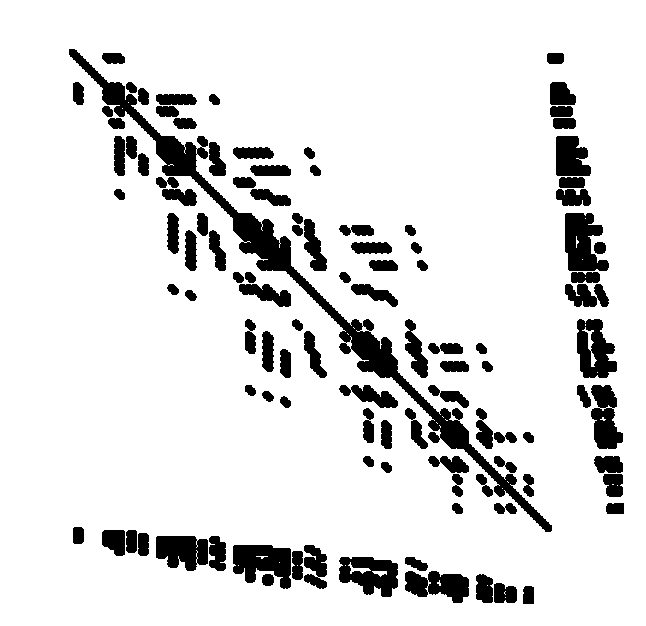
\includegraphics[width=0.5\textwidth]{figs/Kstokes.pdf}
\end{center}
\end{itemize}
\end{frame}


\begin{frame}{eigenvalues for Stokes}

\begin{itemize}
\item FIXME
\begin{center}
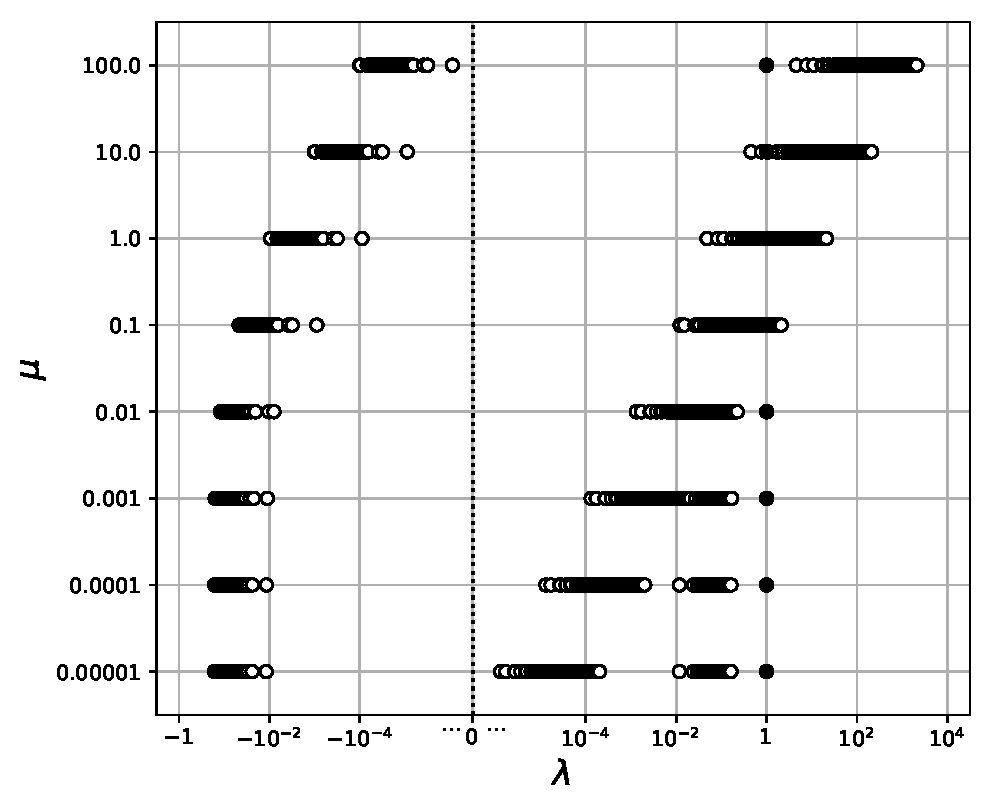
\includegraphics[width=0.5\textwidth]{figs/stokesmueigs.pdf}
\end{center}
\end{itemize}
\end{frame}


\begin{frame}{iterative linear methods}

\hfill 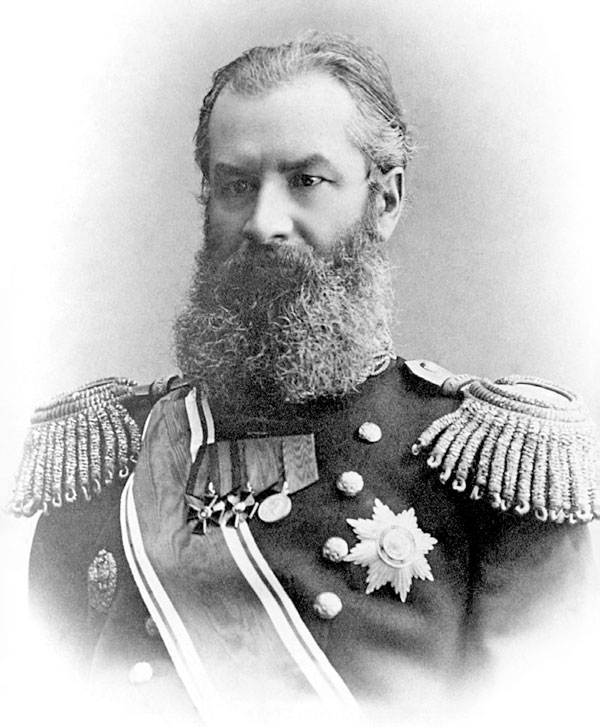
\includegraphics[width=0.25\textwidth]{figs/people/akrylov.jpg}

\vspace{-20mm}
\begin{itemize}
\item FIXME
\end{itemize}
\end{frame}


\begin{frame}{lid-driven cavity convergence}

\begin{itemize}
\item FIXME
\begin{center}
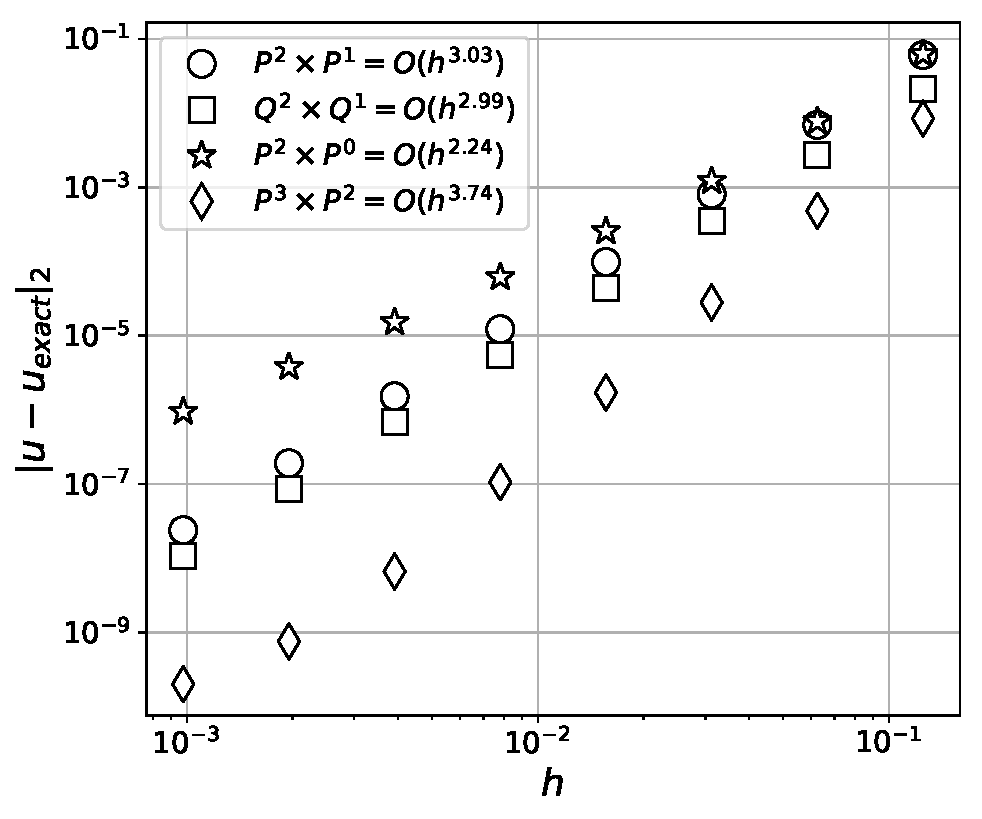
\includegraphics[width=0.5\textwidth]{figs/stokesconv-uerr.pdf}
\end{center}
\end{itemize}
\end{frame}


\section{waves of salad dressing}

\begin{frame}{FIXME}

\begin{itemize}
\item FIXME
\end{itemize}
\end{frame}


\begin{frame}{iterative nonlinear methods}

\hfill 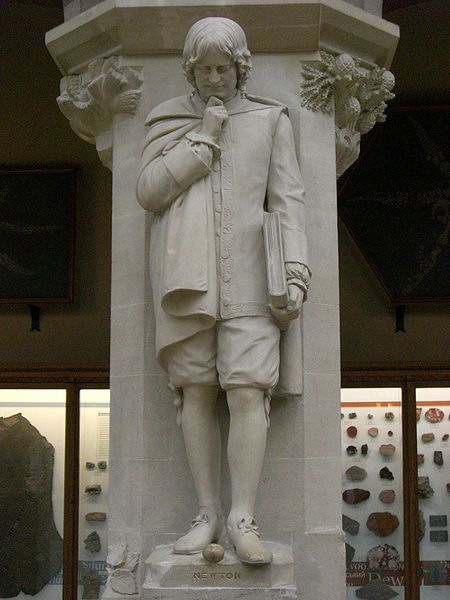
\includegraphics[width=0.25\textwidth]{figs/people/inewton.jpg}

\vspace{-20mm}
\begin{itemize}
\item FIXME
\end{itemize}
\end{frame}


\section{solver performance}

\begin{frame}{FIXME}

\begin{itemize}
\item FIXME
\end{itemize}
\end{frame}

\begin{frame}{multigrid}

\hfill 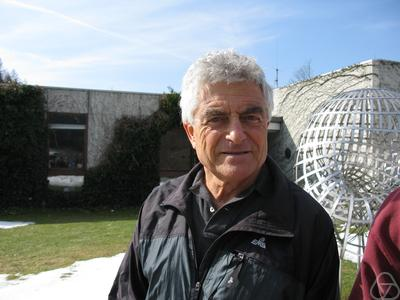
\includegraphics[width=0.25\textwidth]{figs/people/abrandt.jpg}

%\vspace{-20mm}
\begin{itemize}
\item stalling numerical processes must be wrong (\emph{Achi Brandt})
\item FIXME
\end{itemize}
\end{frame}

\begin{frame}{lid-driven cavity optimality}

\begin{itemize}
\item FIXME
\begin{center}
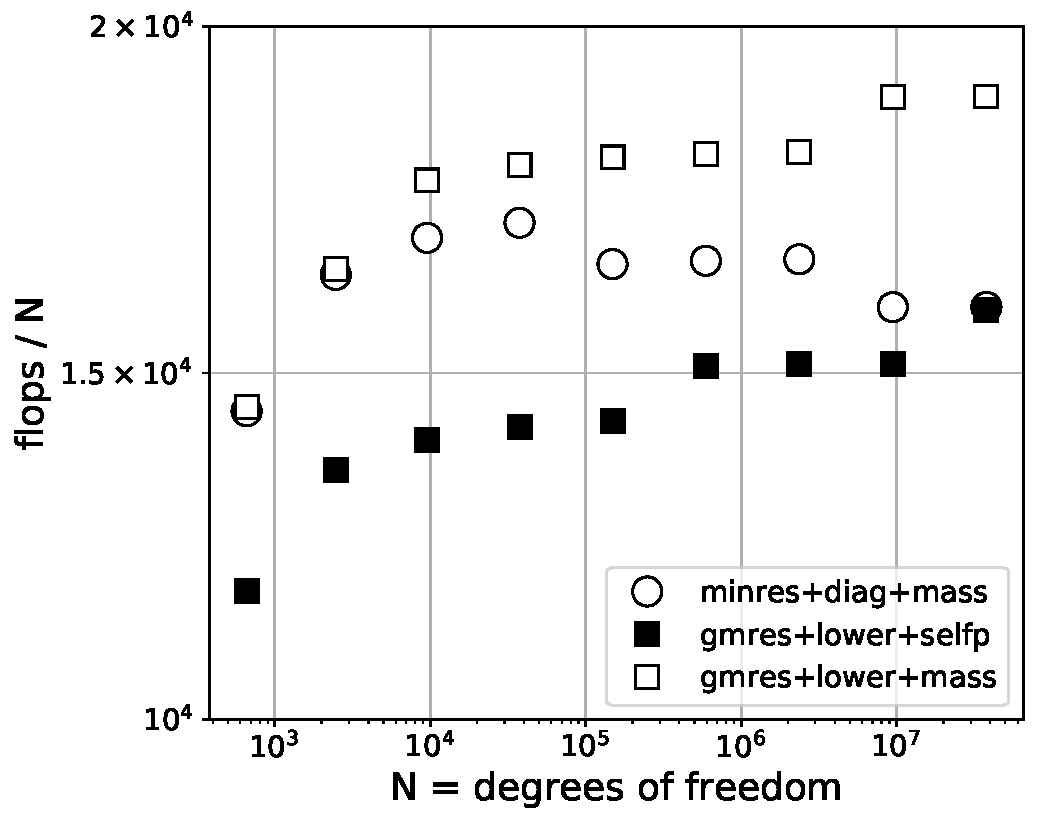
\includegraphics[width=0.5\textwidth]{figs/stokesopt-work.pdf}
\end{center}
\end{itemize}
\end{frame}


\begin{frame}{resolution results}

\begin{itemize}
\item FIXME
\begin{center}
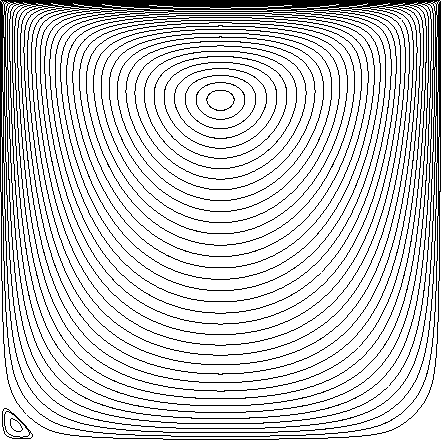
\includegraphics[width=0.25\textwidth]{figs/eddies1.png} \qquad 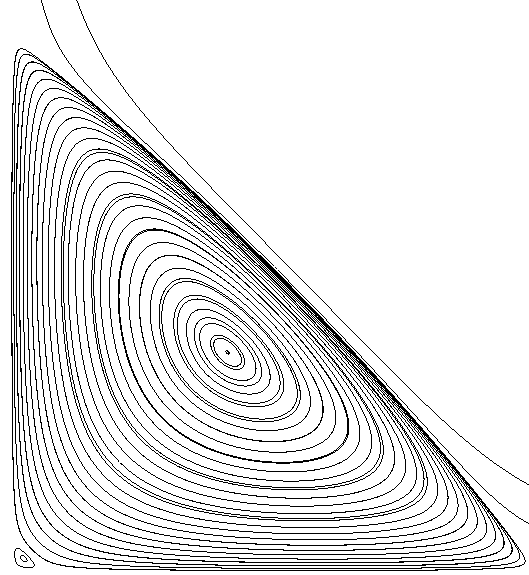
\includegraphics[width=0.25\textwidth]{figs/eddies2.png} \qquad 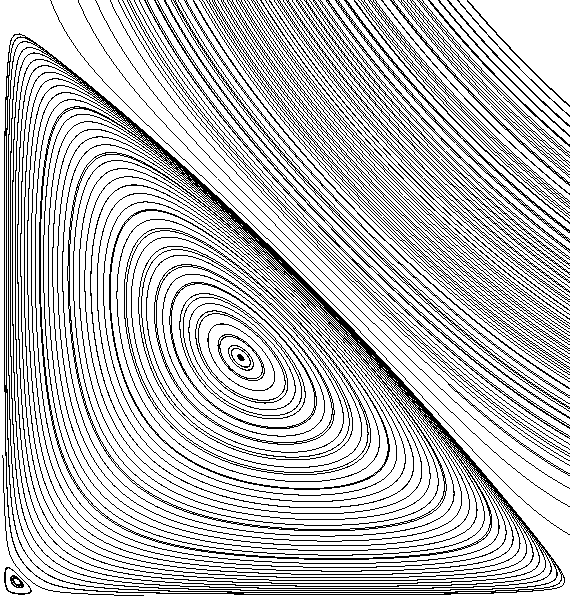
\includegraphics[width=0.25\textwidth]{figs/eddies3.png}
\end{center}
\end{itemize}
\end{frame}


 
\section{ice sheets}

\begin{frame}{FIXME}

\begin{itemize}
\item FIXME
\end{itemize}
\end{frame}


\section{medium flows}

\begin{frame}{Navier-Stokes}

\hfill 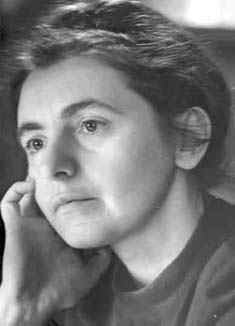
\includegraphics[width=0.25\textwidth]{figs/people/oladyzhenskaya.jpg}

\vspace{-20mm}
\begin{itemize}
\item FIXME
\end{itemize}
\end{frame}


\begin{frame}{references}
\begin{itemize}
\item Elman
\item E.~Bueler, \emph{PETSc for Partial Differential Equations: Numerical Solutions in C and Python}, SIAM Press, 2021
\end{itemize}
\end{frame}


\end{document}

